%  LaTeX support: latex@mdpi.com 
%  For support, please attach all files needed for compiling as well as the log file, and specify your operating system, LaTeX version, and LaTeX editor.

%=================================================================
\documentclass[forecasting,article,submit,pdftex,moreauthors]{Definitions/mdpi}
%\documentclass[preprints,article,submit,pdftex,moreauthors]{Definitions/mdpi}
% For posting an early version of this manuscript as a preprint, you may use "preprints" as the journal. Changing "submit" to "accept" before posting will remove line numbers.

%--------------------
% Class Options:
%--------------------
%----------
% journal
%----------
% Choose between the following MDPI journals:
% accountaudit, acoustics, actuators, addictions, adhesives, adolescents, aerobiology, aerospace, agriculture, agriengineering, agrochemicals, agronomy, ai, aichem, aieng, aimater, aimed, aipa, air, aisens, algorithms, allergies, alloys, amh, analog, analytica, analytics, anatomia, anesthres, animals, antibiotics, antibodies, antioxidants, applbiosci, appliedchem, appliedmath, appliedphys, applmech, applmicrobiol, applnano, applsci, aquacj, architecture, arm, arthropoda, asc, asi, astronautics, astronomy, atmosphere, atoms, audiolres, automation, axioms, bacteria, batteries, bdcc, beverages, biochem, bioengineering, biologics, biology, biomass, biomechanics, biomed, biomedicines, biomedinformatics, biomimetics, biomolecules, biophysica, bioresourbioprod, biosensors, biosphere, biotech, birds, blockchains, bloods, blsf, brainsci, breath, buildings, cancers, carbon, cardio, cardiogenetics, cardiovascmed, catalysts, cells, ceramics, challenges, chemengineering, chemistry, chemosensors, chemproc, children, chips, cimb, civileng, cleantechnol, climate, clinbioenerg, clinpract, clockssleep, cmd, cmtr, coasts, coatings, colloids, colorants, commodities, complexities, complications, compounds, computation, computers, condensedmatter, conservation, constrmater, cosmetics, covid, crops, cryo, cryptography, crystals, csmf, ctn, culture, curroncol, cyber, dairy, data, ddc, dentistry, dermato, dermatopathology, designs, devices, dhi, diabetology, diagnostics, dietetics, digital, disabilities, diseases, diversity, dna, drones, dynamics, earth, ebj, ecm, ecologies, edm, eesp, electricity, electrochem, electronicmat, electronics, encyclopedia, endocrines, energies, eng, engproc, entomology, entropy, environments, environremediat, epidemiologia, epigenomes, esa, est, fermentation, fibers, fintech, fire, fishes, fluids, foods, forecasting, forensicsci, forests, fossstud, foundations, fractalfract, fuels, future, futureinternet, futurepharmacol, futurephys, futuretransp, galaxies, gases, gastroent, gastrointestdisord, gastronomy, gels, genes, geographies, geohazards, geomatics, geometry, geosciences, geotechnics, geriatrics, germs, glacies, grasses, green, greenhealth, gucdd, hardware, hazardousmatters, healthcare, hearts, hemato, hematolrep, hep, heritage, higheredu, highthroughput, horticulturae, hospitals, hydrobiology, hydrogen, hydrology, hydropower, hygiene, idr, iic, ijem, ijerph, ijgi, ijmd, ijms, ijns, ijom, ijpb, ijt, ijtm, ijtpp, ime, immuno, informatics, information, infrastructures, inorganics, insects, instruments, inventions, iot, j, jaestheticmed, jal, jcdd, jcm, jcp, jcrm, jcs, jcto, jdad, jdb, jdream, jemr, jeta, jfb, jfmk, jgbg, jgg, jimaging, jlpea, jmahp, jmmp, jmms, jmp, jmse, jne, jnt, jof, joi, joitmc, joma, jop, joptm, jor, jox, jpbi, jphytomed, jpm, jsan, jtaer, jvd, jzbg, kidneydial, kinasesphosphatases, knowledge, labmed, laboratories, lae, land, life, lights, limnolrev, lipidology, liquids, livers, logics, logistics, lubricants, lymphatics, machines, macromol, magnetism, magnetochemistry, make, marinedrugs, materials, materproc, mathematics, mca, measurements, medicina, medicines, medsci, membranes, merits, metabolites, metals, meteorology, methane, metrics, metrology, micro, microarrays, microbiolres, microelectronics, micromachines, microorganisms, microplastics, microwave, minerals, mining, mmphys, modelling, molbank, molecules, mps, msf, mti, multimedia, muscles, nanoenergyadv, nanomanufacturing, nanomaterials, ncrna, ndt, network, neuroglia, neuroimaging, neurolint, neurosci, nitrogen, notspecified, nursrep, nutraceuticals, nutrients, obesities, occuphealth, oceans, ohbm, onco, optics, oral, organics, organoids, osteology, oxygen, pandemics, parasites, parasitologia, particles, pathogens, pathophysiology, pediatrrep, pets, pharmaceuticals, pharmaceutics, pharmacoepidemiology, pharmacy, philosophies, photochem, photonics, phycology, physchem, physics, physiologia, plants, plasma, platforms, pollutants, polymers, polysaccharides, populations, poultry, powders, precipitation, precisoncol, preprints, proceedings, processes, prosthesis, proteomes, psf, psychiatryint, psychoactives, purification, quantumrep, quaternary, qubs, radiation, rdt, reactions, realestate, receptors, recycling, regeneration, remotesensing, reports, reprodmed, resources, rheumato, rjpm, robotics, rsee, ruminants, safety, sci, scipharm, sclerosis, seeds, sensors, separations, sexes, shi, signals, sinusitis, siuj, skins, smartcities, sna, societies, software, soilsystems, solar, solids, spectroscj, sports, standards, stats, std, stratsediment, stresses, surfaces, surgeries, suschem, sustainability, symmetry, synbio, systems, tae, targets, taxonomy, technologies, telecom, test, textiles, thalassrep, therapeutics, thermo, timespace, tomography, toxics, toxins, tph, transplantology, transportation, traumacare, traumas, tri, tropicalmed, universe, urbansci, uro, vaccines, vehicles, venereology, vetsci, vibration, virtualworlds, viruses, vision, waste, water, welding, wem, wevj, wild, wind, women, world, zoonoticdis

%---------
% article
%---------
% The default type of manuscript is "article", but can be replaced by: 
% abstract, addendum, article, benchmark, book, bookreview, briefcommunication, briefreport, casereport, changes, clinicopathologicalchallenge, comment, commentary, communication, conceptpaper, conferenceproceedings, correction, conferencereport, creative, datadescriptor, discussion, entry, expressionofconcern, extendedabstract, editorial, essay, erratum, fieldguide, hypothesis, interestingimages, letter, meetingreport, monograph, newbookreceived, obituary, opinion, proceedingpaper, projectreport, reply, retraction, review, perspective, protocol, shortnote, studyprotocol, supfile, systematicreview, technicalnote, viewpoint, guidelines, registeredreport, tutorial,  giantsinurology, urologyaroundtheworld
% supfile = supplementary materials

%----------
% submit
%----------
% The class option "submit" will be changed to "accept" by the Editorial Office when the paper is accepted. This will only make changes to the frontpage (e.g., the logo of the journal will get visible), the headings, and the copyright information. Also, line numbering will be removed. Journal info and pagination for accepted papers will also be assigned by the Editorial Office.

%------------------
% moreauthors
%------------------
% If there is only one author the class option oneauthor should be used. Otherwise use the class option moreauthors.

%---------
% pdftex
%---------
% The option pdftex is for use with pdfLaTeX. Remove "pdftex" for (1) compiling with LaTeX & dvi2pdf (if eps figures are used) or for (2) compiling with XeLaTeX.

%=================================================================
% MDPI internal commands - do not modify
\firstpage{1} 
\makeatletter 
\setcounter{page}{\@firstpage} 
\makeatother
\pubvolume{1}
\issuenum{1}
\articlenumber{0}
\pubyear{2026}
\copyrightyear{2026}
%\externaleditor{Firstname Lastname} % More than 1 editor, please add `` and '' before the last editor name
\datereceived{ } 
\daterevised{ } % Comment out if no revised date
\dateaccepted{ } 
\datepublished{ } 
%\datecorrected{} % For corrected papers: "Corrected: XXX" date in the original paper.
%\dateretracted{} % For retracted papers: "Retracted: XXX" date in the original paper.
%\doinum{} % Used for some special journals, like molbank
%\pdfoutput=1 % Uncommented for upload to arXiv.org
%\CorrStatement{yes}  % For updates
%\longauthorlist{yes} % For many authors that exceed the left citation part
%\IsAssociation{yes} % For association journals

%=================================================================
% Add packages and commands here. The following packages are loaded in our class file: fontenc, inputenc, calc, indentfirst, fancyhdr, graphicx, epstopdf, lastpage, ifthen, float, amsmath, amssymb, lineno, setspace, enumitem, mathpazo, booktabs, titlesec, etoolbox, tabto, xcolor, colortbl, soul, multirow, microtype, tikz, totcount, changepage, attrib, upgreek, array, tabularx, pbox, ragged2e, tocloft, marginnote, marginfix, enotez, amsthm, natbib, hyperref, cleveref, scrextend, url, geometry, newfloat, caption, draftwatermark, seqsplit
% cleveref: load \crefname definitions after \begin{document}

%=================================================================
% Please use the following mathematics environments: Theorem, Lemma, Corollary, Proposition, Characterization, Property, Problem, Example, ExamplesandDefinitions, Hypothesis, Remark, Definition, Notation, Assumption
%% For proofs, please use the proof environment (the amsthm package is loaded by the MDPI class).

%=================================================================
% Full title of the paper (Capitalized)
\Title{Automated Demand Forecasting Through Feature-Based Model Selection: Development and Validation of a Computational Tool}

% Author Orchid ID: enter ID or remove command
%\newcommand{\orcidauthorA}{0000-0000-0000-000X}
%\newcommand{\orcidauthorB}{0000-0000-0000-000X}

% Authors, for the paper (add full first names)
\Author{Catalina Valles Gonz\'alez $^{1}$, Joseph Javier S\'anchez Acu\~na $^{1}$, Mar\'ia Paula Corral Ram\'irez $^{1}$, Luis Tarazona-Torres $^{1,}$* and David \'Alvarez-Mart\'inez $^{1}$}

%\longauthorlist{yes}

% MDPI internal command: Authors, for metadata in PDF
\AuthorNames{Catalina Valles Gonzalez, Joseph Javier Sanchez Acuna, Maria Paula Corral Ramirez, Luis Tarazona-Torres and David Alvarez-Martinez}

% Affiliations / Addresses (Add [1] after \address if there is only one affiliation.)
\address{%
$^{1}$ \quad Department of Industrial Engineering, Universidad de los Andes, Bogota 111711, Colombia}

% Contact information of the corresponding author
\corres{Correspondence: ltarazonatorres@gmail.com}

% Current address and/or shared authorship
%\firstnote{Current address: Affiliation.}  
% Current address should not be the same as any items in the Affiliation section.

%\secondnote{These authors contributed equally to this work.}
% The commands \thirdnote{} till \eighthnote{} are available for further notes.

%\simplesumm{} % Simple summary

%\conference{} % An extended version of a conference paper

% Abstract (Do not insert blank lines, i.e. \\)
\abstract{Demand forecasting for short industrial histories (24--48 monthly observations) is often left to manually computed moving averages with no systematic error evaluation. This study develops and validates a computational tool for this regime, built around a validation protocol: structural classification tests calibrated for short, autocorrelated series, a strict separation between hyperparameter tuning and reported performance, and a mandatory naive benchmark. A dedicated analysis quantifies each safeguard's effect: a circular selection-vs-naive comparison inflates the apparent win rate from 63\% to 100\%, and an uncalibrated trend test's 74.4\% false-positive rate is held to a mean of 8.9\% by the sequential test adopted here. Under this protocol, the tool improves on a reference company's incumbent moving average by a median of 19.9\% in scaled error (MASE) on a synthetic panel reflecting its demand structure, beats a naive benchmark on 63\% of 150 public short time series (Wilcoxon W=2127.0,\ p<0.001), and beats Prophet and LightGBM on most series across a range of lengths, though its margin over Prophet is markedly less robust to resampling than its margin over LightGBM. The open-source Python/Dash framework automates structurally-aware model selection, prediction intervals, and inventory-policy parameters end to end, backed by a 276-test suite, with every result reproducible from one seeded command.}

% Keywords
\keyword{Demand forecasting; time series; short-history forecasting; feature-based model selection; nested cross-validation; MASE; walk-forward validation; Prophet; LightGBM; production planning; inventory policy; open-source software.}

% The fields PACS, MSC, and JEL may be left empty or commented out if not applicable
%\PACS{J0101}
%\MSC{}
%\JEL{}

%%%%%%%%%%%%%%%%%%%%%%%%%%%%%%%%%%%%%%%%%%
% Only for the journal Diversity
%\LSID{\url{http://}}

%%%%%%%%%%%%%%%%%%%%%%%%%%%%%%%%%%%%%%%%%%
% Only for the journal Applied Sciences
%\featuredapplication{Authors are encouraged to provide a concise description of the specific application or a potential application of the work. This section is not mandatory.}
%%%%%%%%%%%%%%%%%%%%%%%%%%%%%%%%%%%%%%%%%%

%%%%%%%%%%%%%%%%%%%%%%%%%%%%%%%%%%%%%%%%%%
% Only for the journal Data
%\dataset{DOI number or link to the deposited data set if the data set is published separately. If the data set shall be published as a supplement to this paper, this field will be filled by the journal editors. In this case, please submit the data set as a supplement.}
%\datasetlicense{License under which the data set is made available (CC0, CC-BY, CC-BY-SA, CC-BY-NC, etc.)}

%%%%%%%%%%%%%%%%%%%%%%%%%%%%%%%%%%%%%%%%%%
% Only for the journal BioTech, Fishes, Neuroimaging and Toxins
%\keycontribution{The breakthroughs or highlights of the manuscript. Authors can write one or two sentences to describe the most important part of the paper.}

%%%%%%%%%%%%%%%%%%%%%%%%%%%%%%%%%%%%%%%%%%
% Only for the journal Encyclopedia
%\encyclopediadef{For entry manuscripts only: please provide a brief overview of the entry title instead of an abstract.}

%%%%%%%%%%%%%%%%%%%%%%%%%%%%%%%%%%%%%%%%%%
% Different journals have different requirements. Please check the specific journal guidelines in the "Instructions for Authors" on the journal's official website.
\addhighlights{yes}
\renewcommand{\addhighlights}{%

\noindent
\textbf{What are the main findings?}
 \begin{itemize}[labelsep=2.5mm,topsep=-3pt]
 \item An open-source tool that automates feature-based forecasting method selection for short industrial demand histories improves on an incumbent moving average by a median of 19.9\% in scaled error and beats a naive benchmark on 63\% of 150 public short time series (Wilcoxon $p<0.001$).
 \item Benchmarked under the same leakage-free, three-block protocol against Prophet and LightGBM on 50 series (5 structural regimes $\times$ 10 lengths, 24--180 observations), the tool attains the lowest overall median MASE (0.747 vs.\ 0.785 and 0.893), while a global LightGBM model wins specifically on flat and on zero-inflated, erratic series.
 \end{itemize}\vspace{3pt}
\textbf{What are the implications of the main findings?}
 \begin{itemize}[labelsep=2.5mm,topsep=-3pt]
 \item Structural classification tests calibrated for short samples, together with a strict separation between the blocks used to tune, to select, and to report, are what make an automated forecasting tool's accuracy claims interpretable; both are reusable in any short-history forecasting pipeline.
 \item The regime-dependent result argues for admitting a global gradient-boosting comparator into the candidate pool specifically for zero-inflated, project-driven demand, rather than treating the absence of machine learning as a blanket, undifferentiated limitation.
 \end{itemize}
}

%%%%%%%%%%%%%%%%%%%%%%%%%%%%%%%%%%%%%%%%%%
\begin{document}

%%%%%%%%%%%%%%%%%%%%%%%%%%%%%%%%%%%%%%%%%%
\section{Introduction}

Demand planning plays a central role in operations management, particularly in environments where production, procurement, and inventory decisions depend on anticipatory information. In increasingly dynamic markets characterized by volatility, global competition, and evolving consumption patterns, forecasting future demand becomes both complex and indispensable \cite{mentzer2001,chopra2021}. Accurate forecasting reduces uncertainty, improves resource allocation, and mitigates operational imbalances. However, demand rarely follows perfectly stable patterns. Seasonality, structural variability, irregular consumption behavior, and external shocks limit predictive precision and challenge traditional forecasting methods \cite{makridakis1998,hyndman2021}.

The importance of forecasting in logistics and inventory systems has been extensively documented. Forecasts directly influence storage decisions, transportation planning, procurement policies, and safety stock levels \cite{ballou2004}. Persistent forecast errors may generate overstocks, stockouts, and service-level instability \cite{silver1998}. This is particularly acute for intermittent demand, where a large share of periods have zero or near-zero observed demand and conventional percentage-based errors are undefined or unstable \cite{syntetos2005}. Recent applied evidence indicates that improving forecast accuracy translates into measurable reductions in inventory-related costs \cite{sattar2025}.

From a methodological perspective, classical time-series models such as moving averages, exponential smoothing, regression models, and ARIMA-based approaches remain widely used due to their interpretability and their ability to capture trend and seasonality components \cite{makridakis1998,nahmias2015,hyndman2021}.

Despite methodological advances, organizational practice often lags behind academic development. Kerkk\"{a}nen et al. \cite{kerkkanen2009} report that a substantial share of companies fail to systematically measure forecast errors, which weakens the integration between forecasting and operational planning. This gap between theoretical capability and practical implementation remains a persistent challenge in supply chain management, and it is precisely the gap that motivates the diagnosis reported in this study at a reference plastics manufacturing company.

At the same time, the literature reflects diverging perspectives on the superiority of complex models over simpler statistical techniques. Large-scale forecasting competitions have repeatedly shown that, in many contexts, relatively simple statistical methods perform comparably to, or better than, more sophisticated approaches, and that forecasting performance is strongly conditioned by the structural features of each series \cite{makridakis2018,makridakis2020}. Feature-based model selection --- using structural characteristics such as trend strength, seasonal strength, and stationarity to restrict the pool of candidate models before evaluation --- has been shown to improve robustness and reduce the risk of applying a structurally inconsistent model to a given series \cite{monteromanso2020,talagala2021}. Conversely, machine learning and hybrid approaches have been reported to outperform classical techniques when larger datasets and nonlinear patterns are available \cite{carbonneau2008}. This ongoing debate reinforces the need for systematic, structurally-aware model comparison rather than the uniform application of a single technique across heterogeneous series.

Recent applications also show that automating the interaction between multiple forecasting techniques and interactive visual environments improves the interpretability of both the historical fit and the projected uncertainty for non-expert users \cite{maack2024}, and that this kind of decision-support automation has direct value in transportation and inventory contexts \cite{hernandez2025,nunez2024}. Related Colombian evidence further shows that the choice of forecasting method materially changes downstream planning costs \cite{cubides2025}, reinforcing that method selection is not a peripheral implementation detail.

In this context, this study addresses the following research question: under a regime of short, industrial demand histories (24--48 monthly observations), which classical forecasting methods provide the most reliable out-of-sample performance when method and hyperparameter selection are kept strictly separated from the reported evaluation, and how much of that performance can be attributed to structural, feature-based model filtering rather than to an unconstrained comparison of all candidate methods? To answer this question, nine classical forecasting methods are implemented --- simple average, moving average, weighted moving average, simple exponential smoothing, Holt's linear trend, Holt--Winters, linear regression, ARIMA, and SARIMA --- together with two mandatory benchmarks, the naive and seasonal naive methods, and automated AICc-selected ARIMA/ETS/Theta variants \cite{hyndmankhandakar2008,garza2022}. Method comparison uses the Mean Absolute Scaled Error (MASE) as the primary, scale-independent ranking criterion \cite{hyndmankoehler2006}, complemented by MAPE (computed only over non-zero periods), MAD, MSE, and Mean Error (ME) as a bias diagnostic.

This study makes three contributions. First, it specifies a validation protocol for method selection under short-history conditions: structural, feature-based candidate filtering; a nested tuning/evaluation split that keeps hyperparameter selection strictly separate from reported performance; and an additional outer block that keeps the choice of \emph{method} itself, not only its hyperparameters, separate from the benchmark comparison used to judge it --- together with mandatory naive and seasonal naive benchmarks, without which no accuracy figure in this domain is interpretable. Second, Section~\ref{sec:pitfalls} quantifies, in one place, how much each of these safeguards changes the reported conclusions when it is omitted: how a circular method-selection-vs-naive comparison inflates an apparent win rate, how an uncalibrated structural test distorts candidate filtering, how tuning and reporting on the same block understates error, and how an undefined-at-zero accuracy metric silently discards information. Third, the protocol is evaluated with multiple independent sources of empirical evidence --- a public panel of short time series at several truncation lengths, comparisons against automated statistical and machine-learning baselines (Prophet, LightGBM), an ablation of the structural filter itself, and a synthetic panel reproducing the demand structure of a reference industrial company --- rather than resting on a single case series. The resulting open-source computational framework, developed in Python with Dash, automates this protocol end to end, from data validation to prediction intervals and inventory-policy parameters (safety stock, reorder point).

In addition to methodological validation, computational performance is analyzed by measuring processing time as a function of series length under a fixed, documented hardware and software configuration. The principal findings indicate that no single classical method universally dominates across demand structures, that a naive or seasonal naive benchmark is indispensable to interpret any accuracy claim, and that a transparent, structurally-aware automated pipeline is feasible even under the memory and processing constraints of low-cost consumer hardware.

The remainder of this paper is organized as follows. Section~\ref{sec:methods} describes the research methodology, including the structural classification procedure, the honest tuning/evaluation protocol, and the computational design. Section~\ref{sec:results} presents the empirical and computational results, including the comparison against the incumbent method and against a public panel of short series. Section~\ref{sec:discussion} discusses the findings in relation to the existing literature. Section~\ref{sec:conclusions} concludes with implications, limitations, and directions for future research.

%%%%%%%%%%%%%%%%%%%%%%%%%%%%%%%%%%%%%%%%%%
\section{Materials and Methods}
\label{sec:methods}

\subsection{Research Design}

This study follows a quantitative, applied research design aimed at mathematically characterizing demand time series and developing a generalized, honestly-validated computational forecasting framework suitable for real-world operational environments. The research is non-experimental, as historical demand records are analyzed without manipulation of independent variables, and longitudinal, given that monthly time-series data are evaluated over multiple periods to capture structural dynamics. The methodological approach proceeds in three stages: (i) structural components of each series (trend, seasonality, stationarity) are identified using tests calibrated for the short-sample regime typical of industrial demand data; (ii) a computational tool is developed to automate structurally-aware model comparison under a nested tuning/evaluation protocol; and (iii) the resulting framework is validated against the reference company's incumbent method and against a public panel of short time series. Similar applied quantitative approaches are common in demand planning and inventory forecasting research \cite{petropoulos2022}.

\subsection{Data and Experimental Material}
\label{sec:data}

The experimental material consists of monthly demand time series structured with three variables: \texttt{year}, \texttt{month}, and \texttt{demand}, with an optional \texttt{sku} column for multi-product panels. Empirical validation combines (i) a synthetic panel reproducing the demand structure documented in a qualitative diagnosis of the incumbent forecasting process at a plastics manufacturing company (hereafter, the reference company; Section~\ref{sec:diagnosis}), and (ii) a public benchmark panel described in Section~\ref{sec:panel}. The tool itself is fully generalized and accepts any dataset following this structure.

During data loading, the system converts textual or numeric month labels (Spanish, English, or three-letter abbreviations) into a numerical index; detects and reports, rather than silently resolving, duplicated periods, non-numeric demand values, and gaps in the monthly index; and requires the analyst to choose an explicit gap-handling policy (report, linear interpolation, or zero-fill) before any classification or evaluation step runs. Decimal versus thousands-separator ambiguity in numeric fields is resolved explicitly and the assumed convention is logged. If validation fails, the system returns a descriptive error message and blocks further processing, ensuring data integrity and replicability. A minimum of 18 usable observations is required to proceed.

\subsection{Series Classification Procedure}
\label{sec:classification}

Before model comparison, the tool performs structural classification along three dimensions, in a fixed order: seasonality is assessed first, the series is deseasonalized if seasonality is confirmed, and only then is trend assessed on the deseasonalized series; testing trend before removing a strong seasonal component makes the trend test lose power almost completely in short samples.

\begin{itemize}
\item \textbf{Seasonality Detection.} Two independent conditions must both hold: (i) the seasonal strength $F_S = \max\!\big(0,\, 1 - \mathrm{Var}(R_t)/\mathrm{Var}(S_t+R_t)\big)$ computed from an STL decomposition exceeds 0.40 \cite{wang2006}, and (ii) a Kruskal--Wallis test on the detrended residuals, grouped by position within the seasonal cycle, rejects equality of group medians at the 5\% level \cite{kruskal1952}. Requiring both magnitude and significance evidence, rather than a single autocorrelation threshold, is consistent with combined seasonality-testing practice \cite{ollechwebel2020}. Seasonality is only evaluated when at least three complete annual cycles (36 monthly observations) are available; with fewer cycles STL is not identified and the result is reported as \emph{not evaluable} rather than forced to a yes/no answer.
\item \textbf{Trend Detection.} An Augmented Dickey--Fuller (ADF) test with a deterministic-trend specification is applied first \cite{dickeyfuller1979}. If the series is trend-stationary, the slope is estimated with a Cochrane--Orcutt AR(1)-corrected regression \cite{cochraneorcutt1949} and tested at the 5\% level; if the series instead has a unit root, "trend" is reinterpreted as drift and tested on the mean of the first difference with Newey--West heteroskedasticity- and autocorrelation-consistent standard errors \cite{neweywest1987}. Testing the slope of an ordinary least-squares regression directly, without this sequential unit-root check, is severely oversized under autocorrelated demand.
\item \textbf{Stationarity.} The ADF test is confirmed against the Kwiatkowski--Phillips--Schmidt--Shin (KPSS) test, whose null hypothesis is the complementary one \cite{kpss1992}; when the two tests disagree the series is reported as \emph{inconclusive} instead of forcing a binary verdict.
\end{itemize}

Classification results are displayed to the user and are also used to restrict the pool of forecasting methods evaluated for that series (Section~\ref{sec:methodsincluded}), consistent with feature-based model selection practice \cite{monteromanso2020,talagala2021}: methods that produce a constant-level forecast are only admitted when the series shows no significant trend \emph{and} is stationary in level, and seasonal methods (Holt--Winters, SARIMA, seasonal naive) are only admitted when seasonality is confirmed under the above criterion.

The size and power of the trend and seasonality tests above were validated by Monte Carlo simulation (1000 replicates per scenario, series lengths of 24, 36, 48, and 120 months; reproducible with \texttt{codigo/experimentos/montecarlo\_clasificacion.py}). On white-noise and autocorrelated series with no true trend, the sequential ADF-then-Cochrane--Orcutt test of Section~\ref{sec:classification} falsely reports a trend in a mean of 8.9\% of replicates (maximum 15.8\% across scenarios, the residual driven by the ADF pre-test's own known size distortion at $n=24$), and on series with a real trend but no seasonality, the combined STL-strength-and-Kruskal-Wallis seasonality test falsely reports seasonality in a mean of 1.4\% of replicates (maximum 3.5\%), with statistical power of 100\% to detect true seasonality once at least three full annual cycles are available. Section~\ref{sec:pitfalls} reports these figures alongside those of a naive alternative --- the p-value of an unweighted linear regression for trend and a raw lag-12 autocorrelation threshold for seasonality, both of which this design was chosen to avoid --- to quantify the size distortion that this specification prevents.

\subsection{Forecasting Methods Included}
\label{sec:methodsincluded}

Eleven candidates are implemented: nine classical methods matching the reference company's method inventory --- simple average, moving average, weighted moving average, simple exponential smoothing, Holt's linear trend, Holt--Winters, linear regression, ARIMA, and SARIMA --- plus two mandatory benchmarks, naive (last observed value) and seasonal naive (value observed $m$ periods earlier), without which no accuracy figure is interpretable \cite{hyndmankoehler2006}. ARIMA and SARIMA orders are selected automatically by minimizing the corrected Akaike Information Criterion (AICc) rather than by grid search \cite{hyndmankhandakar2008}, using the \texttt{AutoARIMA} implementation of the \texttt{statsforecast} library \cite{garza2022}; the same library's \texttt{AutoETS} and \texttt{AutoTheta} variants are included as additional automated comparators. Classical model formulations follow Nahmias and Olsen \cite{nahmias2015}. The inclusion of both simple statistical models and automated ARIMA/ETS variants is consistent with evidence from large-scale forecasting competitions that no single method dominates across all demand structures \cite{makridakis2020}.

\subsection{Validation Strategy}
\label{sec:validation}

Model evaluation follows a one-step-ahead rolling-origin (walk-forward) scheme, widely recommended for dependent time-series data \cite{bergmeir2012,tashman2000}. For each admissible origin $t$, every candidate method is fitted using only $y_1,\dots,y_{t-1}$ and produces a one-step-ahead forecast $\hat y_t$; the process repeats across all origins $t \geq \max(10, 2m)$, where $m$ is the seasonal period used by the model. A method that fails to produce a forecast at any origin is excluded from the ranking rather than having its metric averaged over fewer points than its competitors, so that all reported methods are compared on an identical set of origins.

To prevent optimistic bias from hyperparameter selection, the available origins are partitioned into two disjoint, temporally contiguous blocks: an initial \emph{tuning} block, used exclusively to select hyperparameters (grid search for SES, Holt, and Holt--Winters; AICc minimization for ARIMA/SARIMA/ETS/Theta), and a final \emph{evaluation} block of at least eight origins, held out from any hyperparameter search, over which every reported metric is computed. This separation is essential: fitting hyperparameters and reporting performance on the same walk-forward pass, as in an unconstrained grid search evaluated over the same origins used for selection, systematically understates the out-of-sample error.

A further, distinct bias affects any comparison of the selected winning \emph{method} (as opposed to its hyperparameters) against a benchmark: if the naive method is itself one of the candidates over which the winner is chosen by minimum MASE, the winner can never score worse than naive on that same evaluation block, independent of forecasting skill, because the selection is an argmin over a set that includes naive. This is a subtler instance of the same selection-bias family as hyperparameter tuning, and it invalidates a head-to-head "tool vs.\ naive" comparison evaluated on the block that chose the tool's method. For the incumbent-method and public-panel comparisons reported in Section~\ref{sec:incumbente} and Section~\ref{sec:panel}, a third, \emph{outer} block (six origins by default) is therefore reserved beyond the tuning/evaluation split: the entire method-and-hyperparameter-selection protocol above is run on the series truncated to exclude the outer block, and only the resulting winning method is then evaluated, together with the naive and seasonal naive benchmarks, on the outer block that took no part in selecting it (\texttt{forecasting\_core.optimize.honest\_outer\_estimate}). An earlier iteration of this evaluation, before this three-block protocol was implemented, evaluated the winner against naive on the same block that had selected the winner and reported a 100\% win rate on a 150-series panel; that figure was identified as an artifact of the circularity described above before publication and is not reported in this manuscript.

\subsection{Error Metrics}
\label{sec:metrics}

The Mean Absolute Scaled Error is used as the primary ranking criterion, following exactly the definition implemented in \texttt{forecasting\_core.metrics.mase},
\begin{linenomath}
\begin{equation}
\mathrm{MASE} = \frac{\frac{1}{h}\sum_{t=1}^{h}|D_t - F_t|}{\frac{1}{n_{\text{train}}-m}\sum_{t=m+1}^{n_{\text{train}}}|Y_t - Y_{t-m}|},
\end{equation}
\end{linenomath}
where $D_t$ and $F_t$ are the observed and forecast values over the $h$-point held-out evaluation block, and the denominator is the in-sample mean absolute error of the seasonal naive method, computed only on the training block $Y_1,\dots,Y_{n_{\text{train}}}$ that precedes the first evaluation origin --- never on the evaluation block or the full series. Here $m=12$ when the structural classification of Section~\ref{sec:classification} confirms seasonality and $m=1$ otherwise; $m$ is fixed by the series' own structural classification, not a free parameter. This is scale-independent, always defined (including for series with zero-demand periods), and directly interpretable against the seasonal naive benchmark: $\mathrm{MASE}<1$ indicates the model outperforms the naive method in-scale \cite{hyndmankoehler2006}. Mean Absolute Deviation (MAD), Mean Squared Error (MSE), and Mean Absolute Percentage Error (MAPE, computed only over periods with non-zero observed demand, with the count of excluded periods reported) are retained as secondary, interpretable metrics. The Mean Error (ME) is additionally reported as a bias diagnostic --- its sign indicates whether a method systematically under- or over-forecasts, which MAD and MAPE cannot reveal, and which is the quantity that drives systematic stockouts or overstocks rather than the magnitude of the error alone.

\subsection{Hyperparameter Optimization}
\label{sec:hyperopt}

For methods with hyperparameters (SES, Holt, Holt--Winters), a coarse grid is evaluated first over the tuning block only, followed by a bounded local refinement around the best coarse point; grid sizes are capped (at most 27 combinations for Holt--Winters, versus 361 in an unconstrained full-resolution sweep) so that the number of hyperparameter candidates never exceeds the number of tuning origins by more than an order of magnitude. ARIMA and SARIMA no longer use grid search: their order is selected by AICc minimization within \texttt{AutoARIMA}, which removes both the risk of overfitting the tuning block and the combinatorial cost of a $(p,d,q)\times(P,D,Q)$ sweep \cite{hyndmankhandakar2008}.

\subsection{Computational Implementation}
\label{sec:implementation}

Figure~\ref{fig:flowchart} summarizes the end-to-end flow, from data validation through the tuning/evaluation split and the outer-block protocol (Section~\ref{sec:validation}) to the forecast and inventory-policy output described below. The forecasting logic is implemented as a dependency-free Python package (\texttt{codigo/forecasting\_core}) using pandas, NumPy, SciPy, statsmodels, and statsforecast, with no import of the visualization or web layers; a thin Dash/Plotly application consumes this package to provide the interactive interface. This separation makes the statistical logic independently testable: quality control is enforced by an automated test suite of 276 test cases distributed across 13 files (Table~\ref{tab:testsuite}), executed with \texttt{pytest} from the repository root. The suite is not a smoke test: each file targets a specific failure mode the protocol is designed to prevent and, by construction, fails against an implementation lacking the corresponding safeguard and passes against the one adopted here. The most consequential design decision in the suite is that leakage is verified \emph{behaviorally} rather than by code inspection: \texttt{test\_no\_leakage.py} perturbs the observations after a given origin and asserts that the one-step forecast at that origin is bit-for-bit unchanged, a property no model that reads forward in time can satisfy, which makes the guarantee robust to future refactoring in a way that a code review is not. The architecture is modular, matching the four user-facing stages summarized in Table~\ref{tab:stages}: data upload and validation; structural classification and honest method evaluation; hyperparameter optimization under the nested protocol of Section~\ref{sec:hyperopt}; and final forecasting with prediction intervals, tabular export, and inventory-policy parameters (safety stock and reorder point) derived from the empirical distribution of the backtested forecast error.

\begin{table}[H]
\caption{Automated test suite: files, number of collected test cases (\texttt{pytest --collect-only}), and the failure mode each prevents. Executed with \texttt{pytest} from the repository root.\label{tab:testsuite}}
\centering
\begin{tabularx}{\textwidth}{lcX}
\toprule
\textbf{Test file} & \textbf{Tests} & \textbf{Failure mode prevented} \\
\midrule
\texttt{test\_no\_leakage.py} & 42 & A forecast at origin $t$ depending on $y_{\geq t}$; verified by perturbing the future and asserting invariance of the forecast. \\
\texttt{test\_walk\_forward\_parity.py} & 9 & Methods ranked on unequal numbers of origins; silent degradation of a seasonal model to its non-seasonal counterpart; unlogged structural exclusions. \\
\texttt{test\_hyperopt\_no\_bias.py} & 11 & Tuning and evaluation blocks overlapping; a reported metric equal to the minimum of a hyperparameter sweep; an outer-block estimate contaminated by method selection. \\
\texttt{test\_model\_registry.py} & 93 & Substring-based method resolution; silent fallback to a random walk; unbounded hyperparameter grids; loss of any of the eleven candidates from the registry. \\
\texttt{test\_metrics.py} & 15 & MAPE diverging on zero-demand periods; MASE undefined on a constant reference series; ME confused with MAD; non-finite predictions propagating as NaN. \\
\texttt{test\_classification.py} & 24 & Trend or seasonality verdicts inconsistent with the sequential test specification of Section~\ref{sec:classification}; an eligibility rule that no method can satisfy (Section~\ref{sec:pitfalls}). \\
\texttt{test\_data\_loading.py} & 45 & Silent imputation of gaps or duplicates; ambiguous decimal conventions; acceptance of a series too short to validate. \\
\texttt{test\_batch\_memory.py} & 15 & Unbounded memory growth on multi-SKU panels (marked slow; profiled explicitly). \\
\texttt{test\_intervals.py} & 4 & A prediction interval that narrows with the forecast horizon (F31), which has no physical interpretation. \\
\texttt{test\_external\_baselines.py} & 12 & The core suite silently depending on the optional Prophet/\texttt{mlforecast} packages; each is skipped gracefully, by class, when unavailable. \\
\texttt{test\_ablacion\_filtro\_estructural.py} & 1 & The structural-filter ablation of Section~\ref{sec:pitfalls} comparing a different, reordered, or discarded set of series between the filter-on and filter-off runs. \\
\texttt{test\_panel\_publico\_mase\_naive.py} & 2 & The \texttt{mase\_naive} column silently left unpopulated when the winning method is naive itself, which had previously discarded 17 of 150 series from the Wilcoxon test of Section~\ref{sec:panel}. \\
\texttt{test\_vs\_incumbente\_wtl.py} & 3 & An incorrect win/tie/loss breakdown against the incumbent, verified against a hand-solved case. \\
\midrule
\textbf{Total} & \textbf{276} & \\
\bottomrule
\end{tabularx}
\end{table}

Prediction intervals are constructed from empirical quantiles of the walk-forward forecast error at each horizon $h$ (up to \texttt{n\_origins}$=10$ backtest origins), rather than from an analytic formula that would assume normality or a model-specific predictive distribution; when fewer than eight origins are available at a given horizon, the interval falls back to a documented normal--$\sqrt{h}$ approximation, and the tool reports explicitly which of the two methods was used. Because either source of a horizon's interval width is itself an estimate from a small sample, the raw per-horizon width is not guaranteed to grow monotonically with $h$; the tool enforces $\sigma_h \geq \max(\sigma_h^{\text{empirical}},\, \sigma_1\sqrt{h},\, \sigma_{h-1})$ and the corresponding non-decreasing constraint on the interval's total width, so that the reported band never narrows at a longer horizon than at a shorter one purely as an artifact of sampling noise in the backtest.

\begin{table}[H]
\caption{Stages and Components of the Tool\label{tab:stages}}
\centering
\begin{tabularx}{\textwidth}{lX}
\toprule
\textbf{Stage} & \textbf{Components} \\
\midrule
Data loading and validation & Upload the file in .xlsx/.csv format; explicit, non-silent handling of month formats, numeric conventions, duplicates, and temporal gaps; graphical and tabular display of the validated series. \\
Structural classification and honest method evaluation & Sequential seasonality/trend/stationarity classification; feature-based filtering of the candidate pool; nested tuning/evaluation walk-forward ranking by MASE, with every excluded method's reason logged. \\
Hyperparameter optimization & Bounded coarse-to-fine grid search for smoothing methods; AICc-based automatic order selection for ARIMA/SARIMA/ETS/Theta, evaluated only on the tuning block. \\
Forecasting with the selected method & Historical demand, out-of-sample fitted values (never in-sample), and future forecast with an empirical prediction interval; tabular export; derived safety stock and reorder point for a user-specified lead time and service level. \\
\bottomrule
\end{tabularx}
\end{table}

\begin{figure}[H]
    
\includegraphics[width=0.85\textwidth]{figures/flowchart_tool.png}
    \caption{Methodological flow of the forecasting tool: sequential structural classification (seasonality before trend), the tuning/evaluation/outer-block protocol, and the forecast and inventory-policy output.}
    \label{fig:flowchart}
\end{figure}

\subsection{Data, Code, and Availability}
\label{sec:availability}

All computer code associated with this study is publicly available at submission time at \url{https://github.com/GIUSEPPESAN21/Forecasting}, including the dependency-free forecasting package (\texttt{codigo/forecasting\_core}), the Dash application, and the full automated test suite (Table~\ref{tab:testsuite}). Eight reproducibility scripts under \texttt{codigo/experimentos/} generate every quantitative result reported in Section~\ref{sec:results}, each runnable with a single command and a fixed random seed: \texttt{vs\_incumbente.py} and \texttt{panel\_publico.py} for the incumbent and public-panel comparisons; \texttt{benchmark\_tiempos.py} for computational performance; \texttt{montecarlo\_clasificacion.py} for the classification-test validation; \texttt{comparativa\_externa.py} and \texttt{analisis\_sensibilidad\_ci.py} for the external comparison and its sensitivity analysis; and \texttt{ablacion\_filtro\_estructural.py} and \texttt{sensibilidad\_outer\_block.py} for the two robustness checks of Section~\ref{sec:pitfalls}. A versioned release will be archived on Zenodo with a permanent DOI upon acceptance. The reference company's historical sales records that motivated the diagnosis of Section~\ref{sec:diagnosis} are proprietary and are not redistributed; the repository instead ships a synthetic panel that reproduces the structural characteristics documented there (short, volatile, project-driven series with abrupt level changes), so that every script in the repository can be executed end to end without access to any company's data. The public benchmark panel used in Section~\ref{sec:panel} (M3-Monthly) is downloaded automatically by \texttt{codigo/experimentos/panel\_publico.py} from its original public source \cite{makridakis2020m3}.

\subsection{Use of Generative Artificial Intelligence (GenAI)}
\label{sec:genai}
A generative AI system (Claude, Anthropic) was used under direct author supervision to assist in implementing the statistical validation pipeline described in Section~\ref{sec:methods} (structural classification tests, the nested tuning/evaluation protocol, and the prediction-interval and inventory-policy modules), executing the reproducibility scripts that produced the quantitative results reported in Section~\ref{sec:results}, including the Spearman rank-correlation and bootstrap analysis of Section~\ref{sec:sensitivity}, and drafting portions of this manuscript text, based on methodological specifications and literature explicitly selected by the authors. All methodological decisions --- including the choice of MASE as the primary ranking metric, the sequential seasonality-then-trend classification order, the tuning/evaluation split, the inclusion of automated ARIMA/ETS/Theta and external Prophet/LightGBM baselines, and the interpretation of every result reported here, including the explicit finding that the tool's advantage over Prophet is statistically significant but not robust to resampling --- were specified and reviewed by the authors, who bear sole responsibility for it and who independently verified each reported statistic by re-running the accompanying scripts. No automated system was used to generate or fabricate empirical data, company records, or citations; every reference in this manuscript corresponds to a verifiable publication.

%%%%%%%%%%%%%%%%%%%%%%%%%%%%%%%%%%%%%%%%%%
\section{Results}
\label{sec:results}

\subsection{Diagnosis of the Incumbent Forecasting Process}
\label{sec:diagnosis}

A qualitative diagnosis of the forecasting process used by the reference company identified several methodological limitations that motivate this study. Forecasts were produced with a manually computed three-period moving average in spreadsheets, applied uniformly to every product regardless of its trend, seasonality, or stationarity characteristics. No error metric (ME, MAD, MSE, or MAPE) was systematically computed, so the historical accuracy of the incumbent method cannot be assessed from the company's own records, and forecast responsibility was not clearly assigned across products. This is consistent with survey evidence that a large share of firms do not formally evaluate forecast error \cite{kerkkanen2009}. This diagnosis is reported here strictly as \emph{motivation}: it is a qualitative description of a practice, not a numerical accuracy figure for the incumbent method, and it is not itself an evaluated result. The quantitative comparisons that the paper's accuracy claims rest on are the synthetic-panel and public-panel validations of Sections~\ref{sec:incumbente} and~\ref{sec:panel}, which reproduce the demand structure documented here rather than depending on it.

\subsection{Validation of the Structural Classification Tests}
\label{sec:mcvalidation}

Before any accuracy figure can be interpreted, the structural classification step on which every downstream candidate-pool restriction depends (Section~\ref{sec:classification}) must itself be shown to be statistically reliable. Figure~\ref{fig:montecarlo} reports the same Monte Carlo validation summarized in Section~\ref{sec:classification} (1000 replicates per scenario, series lengths of 24, 36, 48, and 120 months; \texttt{codigo/experimentos/montecarlo\_clasificacion.py}), broken down by scenario and length rather than only as the two aggregate rates already cited. Panel (A) shows that the residual false-positive rate of the adopted trend test is not uniform across data-generating processes: it sits close to the nominal 5\% for white noise and for clean trend-free scenarios, but remains elevated for the random-walk scenario (11.7--15.8\% across lengths), a known consequence of the ADF pre-test's reduced power to reject a unit root at these sample sizes rather than a defect of the trend step that follows it. Panel (B) shows the adopted seasonality test at or below its nominal rate in every scenario and at every length for which seasonality is evaluable at all ($n\geq 36$); at $n=24$ seasonality is reported as \emph{not evaluable} by construction (Section~\ref{sec:classification}) and is therefore omitted from the panel rather than assigned a false-positive rate. Panel (C) places the two aggregate rates side by side against the 5\% nominal-size reference: the common shortcuts this design was chosen to avoid --- an unweighted regression $p$-value for trend and a raw lag-12 autocorrelation threshold for seasonality --- reach 74.4\% and 50.2\%, against 8.9\% and 1.4\% for the tests adopted here.

\begin{figure}[H]
    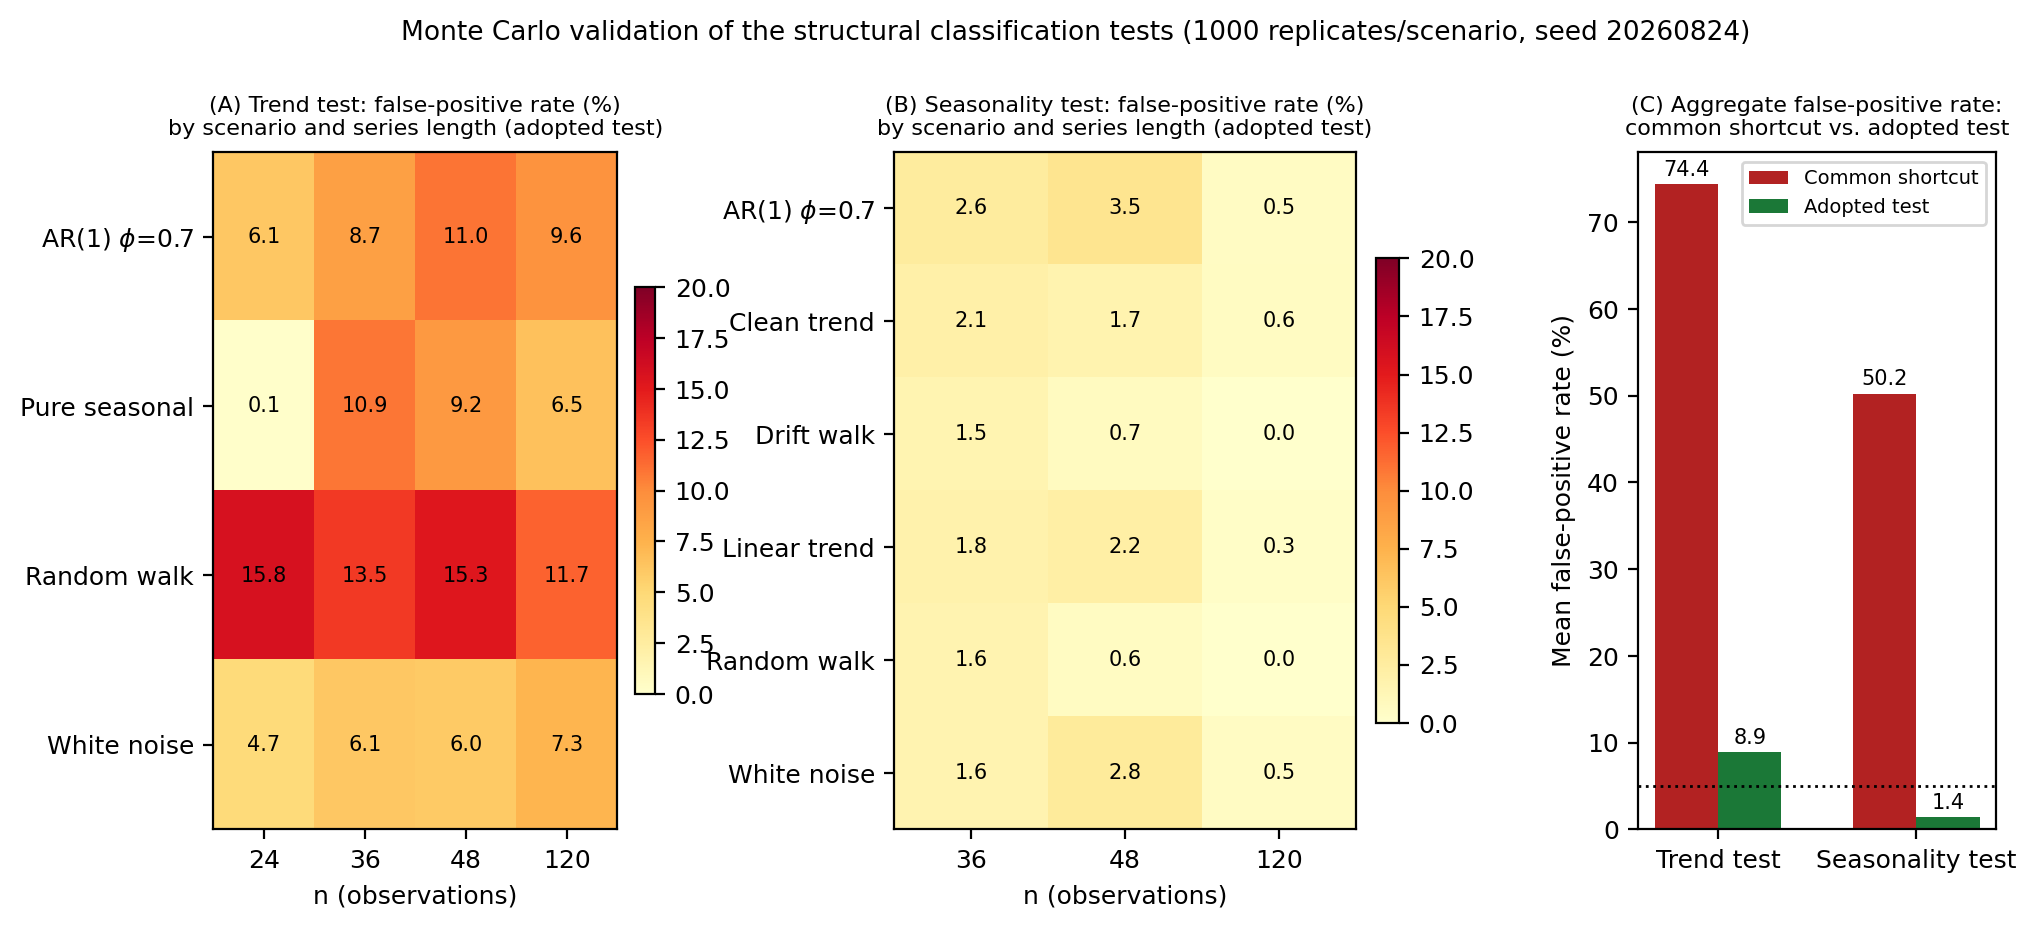
\includegraphics[width=\textwidth]{figures/fig2_montecarlo_clasificacion.png}
    \caption{Monte Carlo validation of the structural classification tests (1000 replicates per scenario, seed 20260824). (A) and (B): false-positive rate of the adopted trend and seasonality tests, respectively, by data-generating scenario (ground truth: no trend / no seasonality) and series length; the $n=24$ column is omitted from Panel (B) because seasonality is not evaluable below three annual cycles. (C) Mean false-positive rate aggregated across scenarios, common shortcut versus adopted test, against the 5\% nominal-size reference (dotted line).}
    \label{fig:montecarlo}
\end{figure}

\subsection{Illustrative Walkthrough of the Tool}
\label{sec:walkthrough}

To illustrate the pipeline end to end, this subsection reports the exact output of the tool on a single 36-month synthetic demand series that reproduces the qualitative characteristics documented in Section~\ref{sec:diagnosis} --- a moderate upward trend, seasonal variation, and abrupt month-to-month changes driven by exogenous demand shocks. The series, and every number reported in this subsection, is produced deterministically by \texttt{codigo/experimentos/caso\_ilustrativo.py} (fixed random seed), so the walkthrough is reproducible with a single command; it is illustrative of tool mechanics and is not a substitute for the incumbent-method and public-panel validations in Sections~\ref{sec:incumbente}--\ref{sec:panel}, which are the results the paper's accuracy claims rest on.

\subsubsection{Data Loading, Validation, and Classification}

Once the series is loaded, the tool confirms 36 valid monthly observations (January 2022 to December 2024) and reports the structural classification: a statistically significant trend (Cochrane--Orcutt-corrected $p<0.001$), confirmed seasonality (STL seasonal strength $F_S=0.752$, Kruskal--Wallis $p=0.031$ on detrended residuals), and a series that is stationary around its deterministic trend once seasonality and trend are accounted for. Because trend is significant, the structural filter of Section~\ref{sec:classification} excludes the three constant-level methods (simple average, moving average, weighted moving average) from the candidate pool, each with its exclusion reason logged rather than silently dropped; because seasonality is confirmed, the seasonal methods remain eligible. Ten candidates are evaluated: naive, seasonal naive, SES, Holt, Holt--Winters, linear regression, and the four AICc-selected automated variants (ARIMA, SARIMA, ETS, Theta).

\subsubsection{Method Evaluation and Selection}

Table~\ref{tab:rankingcaso} reports the ranking on the held-out evaluation block (eight origins, none of which participated in hyperparameter selection), ordered by MASE. The automatically-selected SARIMA model achieves the lowest MASE (0.486), improving on the seasonal naive benchmark (MASE 0.895) by 46\% and on the naive benchmark (MASE 0.935) by 48\%; both mandatory benchmarks are shown explicitly, alongside every other candidate. Every method in the table was evaluated on the identical set of eight origins ($n_{\text{preds}}=8$ throughout), so no comparison in this table is confounded by unequal sample sizes across methods.

\begin{table}[H]
\caption{Out-of-sample ranking for the illustrative series (evaluation block, $n=8$ origins). Values reproduced by \texttt{codigo/experimentos/caso\_ilustrativo.py}.\label{tab:rankingcaso}}
\centering
\begin{tabularx}{\textwidth}{Xccccc}
\toprule
\textbf{Method} & \textbf{MASE} & \textbf{MAPE (\%)} & \textbf{MAD} & \textbf{ME} & \textbf{$n_{\text{preds}}$} \\
\midrule
SARIMA (AICc)               & \textbf{0.486} & 5.83  & 139.3 & 56.2  & 8 \\
Linear regression            & 0.637 & 7.81  & 182.6 & 6.4   & 8 \\
SES                           & 0.659 & 7.74  & 188.8 & 151.7 & 8 \\
ARIMA (AICc)                  & 0.661 & 7.61  & 189.5 & 157.4 & 8 \\
Holt                          & 0.714 & 8.50  & 204.6 & 107.6 & 8 \\
Theta (AICc)                  & 0.759 & 9.20  & 217.5 & 18.7  & 8 \\
ETS (AICc)                    & 0.778 & 9.34  & 223.0 & 40.7  & 8 \\
Seasonal naive                & 0.895 & 10.90 & 256.6 & 243.3 & 8 \\
Naive                         & 0.935 & 11.11 & 268.0 & 65.0  & 8 \\
Holt--Winters                 & 1.201 & 14.64 & 344.2 & 12.3  & 8 \\
\bottomrule
\end{tabularx}
\end{table}

Since SARIMA's order is selected automatically by AICc rather than through a hyperparameter grid, no further tuning step applies (Section~\ref{sec:hyperopt}); this is itself a direct consequence of replacing the original unconstrained $(p,d,q)\times(P,D,Q)$ sweep, which for a series this short would have re-used the same evaluation origins to both select and score the model.

\subsubsection{Forecasting with the Selected Method}

Figure~\ref{fig:forecastcaso} shows the historical demand, the out-of-sample fitted values over the evaluation block (never in-sample), and the 12-month-ahead forecast with its 95\% prediction interval. At this series' length, fewer than the minimum eight backtest origins remain at every horizon, so the interval uses the normal--$\sqrt{h}$ fallback of Section~\ref{sec:implementation} throughout, and the tool reports this explicitly in its output (\texttt{pi.method}) rather than silently defaulting to it. The resulting band widens smoothly and monotonically with the horizon --- from a standard deviation of 360 units at one month ahead to 1248 units at twelve months ahead (\texttt{resultados/caso\_ilustrativo\_pronostico.csv}) --- by construction of the monotonicity constraint described above, rather than as an incidental property of this particular series.

\begin{figure}[H]
    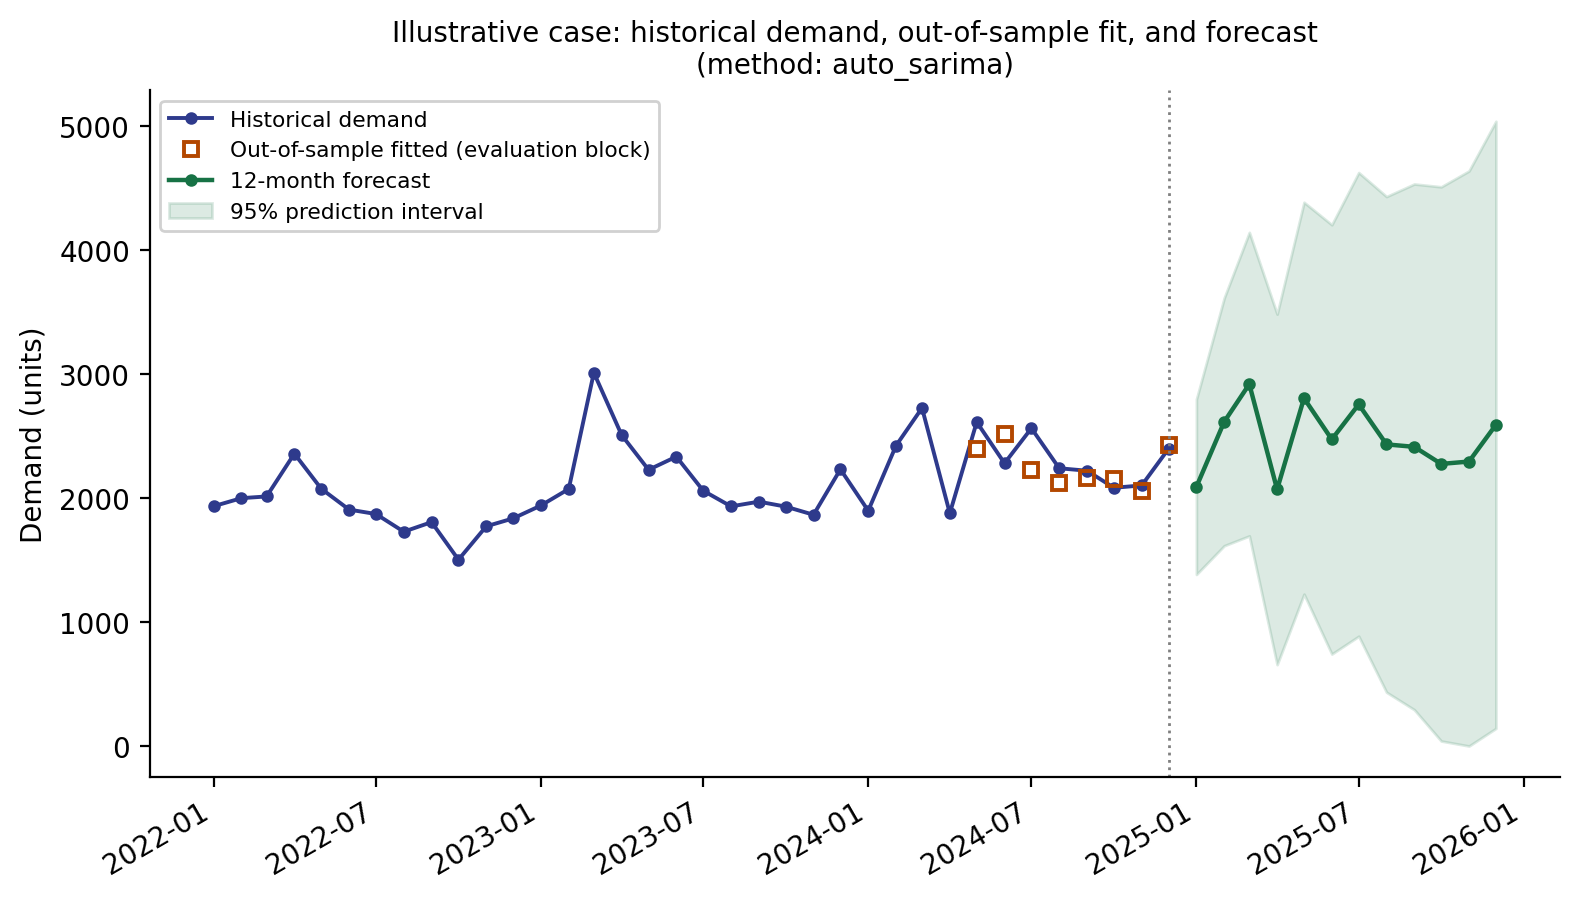
\includegraphics[width=0.85\textwidth]{figures/fig2_forecast_caso.png}
    \caption{Historical demand, out-of-sample fitted values, and 12-month forecast with 95\% prediction interval for the illustrative series (SARIMA, AICc-selected order).}
    \label{fig:forecastcaso}
\end{figure}

\subsubsection{Inventory Policy}

Given a three-month lead time and a 95\% service level, the tool computes safety stock as $\mathrm{SS} = z \cdot \sigma_L$, where $z=\Phi^{-1}(0.95)=1.645$ is the standard-normal quantile for the requested service level and $\sigma_L$ is the standard deviation of the \emph{accumulated} forecast error over the lead time, estimated directly from ten backtest origins of the walk-forward pass (a separate, internal backtest of the safety-stock module, distinct from the eight evaluation-block origins of Table~\ref{tab:rankingcaso}, which score candidate methods against each other rather than accumulate lead-time error) rather than assumed as $\sigma_1\sqrt{L}$, which would understate $\sigma_L$ whenever consecutive forecast errors are correlated. For this series: expected lead-time demand of 7{,}620 units, $\sigma_L=762$ units, $\mathrm{SS}=1{,}253$ units ($1.645 \times 762 \approx 1253$), and a resulting reorder point of 8{,}873 units. This closes the gap between a point forecast and an actionable inventory decision.

\subsection{Comparison Against the Incumbent Method and a Naive Benchmark}
\label{sec:incumbente}

The central claim motivating this study --- that the proposed protocol improves on the reference company's incumbent practice --- is tested directly by reconstructing the incumbent method (a fixed three-period moving average, matching the diagnosis in Section~\ref{sec:diagnosis}) and evaluating both it and the tool's selected method on an \emph{outer} block of origins that participated in neither hyperparameter tuning nor method selection (Section~\ref{sec:validation}, Figure~\ref{fig:flowchart}), over 40 demand series (\texttt{forecasting\_core.optimize.honest\_outer\_estimate}). This outer-block step is necessary because comparing the selected method against naive on the same block used to select it is circular --- naive is one of the candidates the selection argmin runs over, so the selected method can never lose to naive on that specific block by construction, independent of forecasting skill; Section~\ref{sec:pitfalls} quantifies exactly how large this effect is. Because the reference company's historical sales file is not available for this study (Section~\ref{sec:availability}, Data Availability), this comparison is reported on a synthetic panel that reproduces the structural characteristics documented in Section~\ref{sec:diagnosis} (30--42 monthly observations, project-driven volatility, abrupt level changes); the comparison script (\texttt{codigo/experimentos/vs\_incumbente.py}) accepts a real sales file as a direct drop-in replacement (\texttt{--input}), which Section~\ref{sec:discussion} lists among the concrete directions for future work.

Table~\ref{tab:incumbente} summarizes the result. Across the 40 series, the tool's selected method improves on the incumbent by a median per-series reduction in MASE of 19.9\% and outperforms the incumbent on 80\% of series; the improvement of the medians themselves (0.922 to 0.807) is a more conservative 12.5\%, a complementary but non-interchangeable statistic reported here to avoid the ambiguity of citing only one of the two. A paired Wilcoxon signed-rank test on per-series MASE (tool vs.\ incumbent, excluding exact ties) gives $W=94.0,\ p=4.9\times10^{-6}$ ($n=40$), indicating the improvement is unlikely to be sampling noise on this panel. Against the plain naive benchmark, evaluated on the same held-out block, the tool wins on 24 series, ties on 10 (the tool itself selected naive as the winning method), and loses on 6 --- a materially informative breakdown precisely because, under this protocol, none of these three counts is guaranteed by construction. This remains a more modest and more defensible claim than an unqualified statement that the tool "significantly improves accuracy": on this synthetic panel, one in five series see no improvement over the incumbent, most often plain or lightly-noisy series where a three-period moving average is already close to optimal.

\begin{table}[H]
\caption{Tool vs.\ incumbent method vs.\ naive benchmark, evaluated on an outer block held out from both hyperparameter tuning and method selection (40 synthetic series reproducing the reference company's demand structure). Reproducible with \texttt{codigo/experimentos/vs\_incumbente.py --synthetic --n-series 40 --seed 20260824}.\label{tab:incumbente}}
\centering
\begin{tabularx}{\textwidth}{Xccc}
\toprule
\textbf{Metric (median across series)} & \textbf{Incumbent (MA-3)} & \textbf{Naive} & \textbf{Tool (selected method)} \\
\midrule
MASE   & 0.922 & 0.949 & 0.807 \\
MAPE (\%) & 14.4 & 11.4 & 10.1 \\
$|$ME$|$ (bias magnitude) & 217.1 & 55.4 & 111.9 \\
\bottomrule
\end{tabularx}
\end{table}

\subsection{Validation on a Public Panel of Short Time Series}
\label{sec:panel}

A single case-study series cannot support a claim of general superiority: the sampling variance of a MASE estimate over 8--18 backtest origins is large. To provide broader evidence, the full pipeline was run on the same 150-series sample drawn from the M3-Monthly competition panel \cite{makridakis2020m3} (native series span 66--144 observations) truncated to three lengths spanning the regime this tool targets: 24, 36, and 48 observations (\texttt{codigo/experimentos/panel\_publico.py --max-len \{24,36,48\}}). No coverage was silently capped: the pipeline logs an explicit exclusion reason for any series it cannot rank (insufficient history for the outer-block protocol of Section~\ref{sec:validation}, or no eligible candidate after structural filtering). At 24 observations, none of the 150 series retain enough history for the three-block protocol (24 minus a 6-origin outer block leaves 18, below the minimum of 22 the inner tuning/evaluation split requires) and the panel produces zero rankings; at 36 observations, all 150 series rank, with a median MASE of 0.820 against 0.851 for naive and a win rate of 50\%; at 48 observations, the length used for Table~\ref{tab:panel} below, all 150 rank with a median MASE of 0.701 against 0.829 for naive and a win rate of 63\%. Reported accuracy and the tool's margin over naive both improve as more history becomes available, and the shortest part of the regime this tool targets (24--35 observations) is precisely where this specific public panel cannot validate it at all --- a limitation made explicit in Section~\ref{sec:discussion} rather than papered over by reporting only the most favorable length.

\begin{table}[H]
\caption{Median MASE by structural regime on the M3-Monthly panel (truncated to $\leq$48 observations, $n=$150 series). Reproducible with \texttt{codigo/experimentos/panel\_publico.py}.\label{tab:panel}}
\centering
\begin{tabularx}{\textwidth}{Xcccc}
\toprule
\textbf{Structural regime} & \textbf{n series} & \textbf{Naive} & \textbf{Seasonal naive} & \textbf{Tool (selected method)} \\
\midrule
Seasonal + trend & 21 & 1.125 & 1.063 & 0.719 \\
Seasonal, no trend & 31 & 0.940 & 0.916 & 0.665 \\
Trend, no seasonality & 42 & 0.702 & 1.247 & 0.634 \\
Flat (no trend, no seasonality) & 56 & 0.783 & 1.567 & 0.781 \\
\bottomrule
\end{tabularx}
\end{table}

Table~\ref{tab:panel} breaks the result down by structural regime. Of the 150 series, the tool's selected method \emph{is} the naive method on 17 (11\%), which are exact ties by construction; of the remaining 133 series with a non-trivial pairwise comparison, it wins on 95 (63\% of the full 150) and loses on 38 (25\%). A Wilcoxon signed-rank test on these 133 non-tied paired per-series MASE values (tool vs.\ naive) gives $W=2127.0,\ p<0.001$, indicating that the tool's selected method achieves significantly lower MASE than the naive benchmark across the panel. This aggregate result masks regime-level heterogeneity that Table~\ref{tab:panel} makes visible: in the flat regime (no trend, no seasonality), the most numerous in the panel at 56 series, the tool's selected method wins on only 25 series (45\%, 9 ties, 22 losses) even though its \emph{median} MASE is marginally lower than naive's (0.781 vs.\ 0.783) --- a case where the median comparison and the win-rate comparison tell different stories, because a subset of series with a large advantage pulls the median down while naive is more consistently competitive across the rest of the regime. By contrast, in the trend-without-seasonality regime the tool wins on 57\% of series (24 wins, 7 ties, 11 losses) with a wider median margin (0.634 vs.\ 0.702), and in the two seasonal regimes it wins on 81\% and 94\% of series respectively. This is reported as a signed-rank result together with a full win/tie/loss breakdown, a more conservative and more transparent pair of claims than an unreported or single-series accuracy comparison, and Section~\ref{sec:pitfalls} quantifies how different --- and less informative --- the headline number would look under the circular protocol this outer-block design avoids.

\subsection{Computational Performance}
\label{sec:computo}

Processing time was measured with \texttt{time.perf\_counter()} over five repetitions per series length, reporting mean and standard deviation rather than a single run, and including the hyperparameter-tuning stage. All measurements were taken on a single machine (AMD Ryzen 5 7000-series, 8 logical CPUs, 8\,GB RAM, Windows 11 build 26200; Python 3.11.9; pandas 2.2.2; statsmodels 0.14.6; statsforecast 2.1.1) and are exactly reproduced by \texttt{codigo/experimentos/benchmark\_tiempos.py}; results are reported in Table~\ref{tab:tiempos}. This hardware profile is used throughout the paper wherever a hardware description is needed. With only five repetitions per length, the standard deviation at $n=96$ (10.8\,s, driven by one 48.8\,s outlier run) is a noisy estimate rather than a stable characterization of variance. A validation re-run with ten repetitions per length (same seed, same hardware; \texttt{resultados/benchmark\_tiempos\_reps10.csv}) did not resolve this: variance was, if anything, larger (e.g., $n=96$: mean 34.7\,s, SD 19.1\,s, range 20.4--76.1\,s; $n=24$: mean 6.2\,s, SD 7.0\,s, range 2.4--25.2\,s), and the fitted exponent shifted from 1.34 to 1.11. Both measurements agree that $n\leq48$ stays within the 25\,s interactive-session target and that $n=120$ stays within roughly a minute, but neither five nor ten repetitions on this shared, non-isolated consumer machine is enough to pin down a precise scaling exponent or a tight variance estimate; the headline figures reported in Table~\ref{tab:tiempos} should be read as an order-of-magnitude budget check, not as a precision timing benchmark, and this is a limitation of the measurement environment rather than of the pipeline's algorithmic complexity.

\begin{table}[H]
\caption{End-to-end pipeline time (classification, evaluation, hyperparameter tuning, and prediction interval), mean $\pm$ standard deviation over five repetitions per series length.\label{tab:tiempos}}
\centering
\begin{tabularx}{\textwidth}{Xcccc}
\toprule
\textbf{n (observations)} & \textbf{Mean (s)} & \textbf{SD (s)} & \textbf{Min (s)} & \textbf{Max (s)} \\
\midrule
24  & 3.9  & 0.6  & 3.1  & 4.7  \\
48  & 11.8 & 2.6  & 9.5  & 16.2 \\
72  & 15.2 & 2.1  & 12.3 & 17.4 \\
96  & 29.9 & 10.8 & 22.4 & 48.8 \\
120 & 33.3 & 7.1  & 25.4 & 44.3 \\
\bottomrule
\end{tabularx}
\end{table}

An empirical power-law fit, $\text{time} \approx 0.058 \cdot n^{1.34}$, characterizes the growth as superlinear but sub-quadratic. The design target for an interactive session on this hardware profile was a full pipeline run of at most 25\,s for the short-history regime this tool targets ($n\leq48$); both measured lengths in that range meet it (3.9\,s at $n=24$, 11.8\,s at $n=48$). Longer series, up to the 120 observations evaluated here (33.3\,s on average), fall outside that specific target by design --- the target was never intended to bound the full range of series lengths the tool can process, only the short-history case this refactor optimizes for --- and 33.3\,s remains comfortably inside the response-time budget of an interactive session. For reference, a single, non-repeated timing of an earlier, unoptimized version of the pipeline at $n=120$, including the same tuning stage, gave 183\,s; because that figure was not measured with the repeated-trial protocol used for Table~\ref{tab:tiempos}, it is reported here only as an order-of-magnitude reference, not as a directly comparable data point. The improvement relative to that earlier version is primarily attributable to eliminating redundant walk-forward recomputation (Section~\ref{sec:validation}) and to replacing an unconstrained ARIMA/SARIMA grid search with AICc-based automatic order selection (Section~\ref{sec:hyperopt}).

\subsection{Comparison Against External Baselines (Prophet, LightGBM)}
\label{sec:autobaselines}

Beyond the classical and automated-statistical candidates internal to the tool's own pool (Section~\ref{sec:methodsincluded}), the protocol is also compared against two external, popular automated forecasting libraries not included in that pool: Prophet 1.4.0 \cite{taylorletham2018} and a gradient-boosted-tree regressor, LightGBM 4.7.0 \cite{ke2017lightgbm}, wrapped through \texttt{mlforecast} 1.1.0 with lagged-demand and rolling-mean features \cite{garza2022mlforecast}. Both are fitted and evaluated with the same outer-block protocol as the tool's own selected method (\texttt{forecasting\_core.optimize.honest\_outer\_estimate}; \texttt{codigo/external\_baselines}), on a synthetic panel spanning ten series lengths from 24 to 180 monthly observations (five structural regimes $\times$ five seeds per length; \texttt{codigo/experimentos/comparativa\_externa.py}), so that the comparison covers both the short-history regime this tool targets and longer series where a more data-hungry method has more to work with.

\begin{figure}[H]
    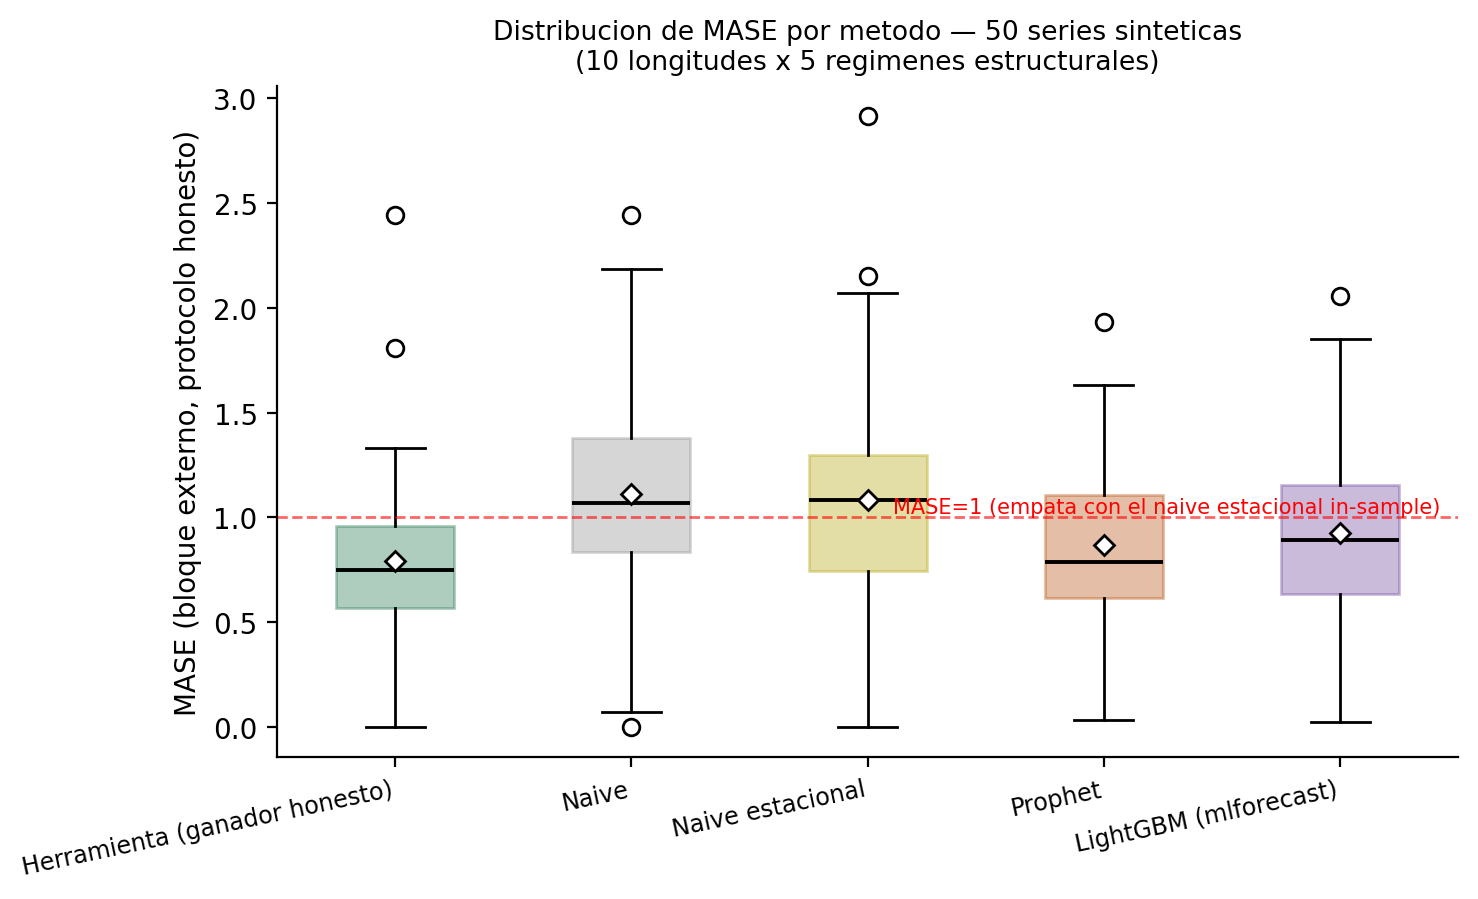
\includegraphics[width=0.85\textwidth]{figures/fig_c1_boxplot_mase.png}
    \caption{Distribution of external-block MASE by method across the 50-series comparison (diamonds mark the mean; the dashed line marks MASE=1, parity with the in-sample seasonal-naive benchmark).}
    \label{fig:boxplotmase}
\end{figure}

Table~\ref{tab:externo} and Figures~\ref{fig:boxplotmase}--\ref{fig:masevslongitud} summarize the result (\texttt{resultados/comparativa\_externa.csv}, 50 series). Across the full panel, the tool's selected method has the lowest median MASE (0.747), ahead of Prophet (0.785) and LightGBM (0.893), and all three outperform the naive benchmark (1.070) on the median series. The tool's selected method outperforms Prophet on 64\% of series (Wilcoxon signed-rank $W=428.0,\ p=0.043$) and LightGBM on 72\% ($W=332.0,\ p=0.003$); both differences are significant at the 5\% level, though the margin against Prophet is markedly narrower. Both external comparators are, in their own right, significantly more accurate than the naive benchmark (Prophet: $W=295.0,\ p<0.001$, 74\% win rate; LightGBM: $W=341.0,\ p=0.004$, 66\% win rate), which indicates that the tool's advantage over them reflects a genuine, if moderate and unevenly robust, margin over two competent comparators rather than an artifact of comparing against artificially weakened baselines. Figure~\ref{fig:boxplotmase} shows the full distribution of external-block MASE by method rather than only its median: the tool has the lowest median and an interquartile range comparable to that of the naive benchmarks, while Prophet and LightGBM show broader upper tails, consistent with a small number of series --- typically the shortest and most erratic --- on which a heavier, more parametrized model overfits a thin tuning history.

This ordering is not uniform across series length, however: at the shortest length evaluated ($n=24$), LightGBM has the lowest median MASE (0.798, against 0.909 for the tool and 0.948 for Prophet), and it is again the strongest method at $n=120$ (0.388); Figure~\ref{fig:masevslongitud} shows the tool's selected method and Prophet crossing LightGBM's median at several intermediate lengths rather than one method dominating throughout. This is consistent with the same competition evidence discussed in Section~\ref{sec:discussion}: no single method, classical or automated, dominates across all regimes and lengths, and a boosted-tree regressor with lag features can be competitive precisely where a longer history gives it enough rows to learn from, even in the moderately short regime this tool targets.

\begin{figure}[H]
    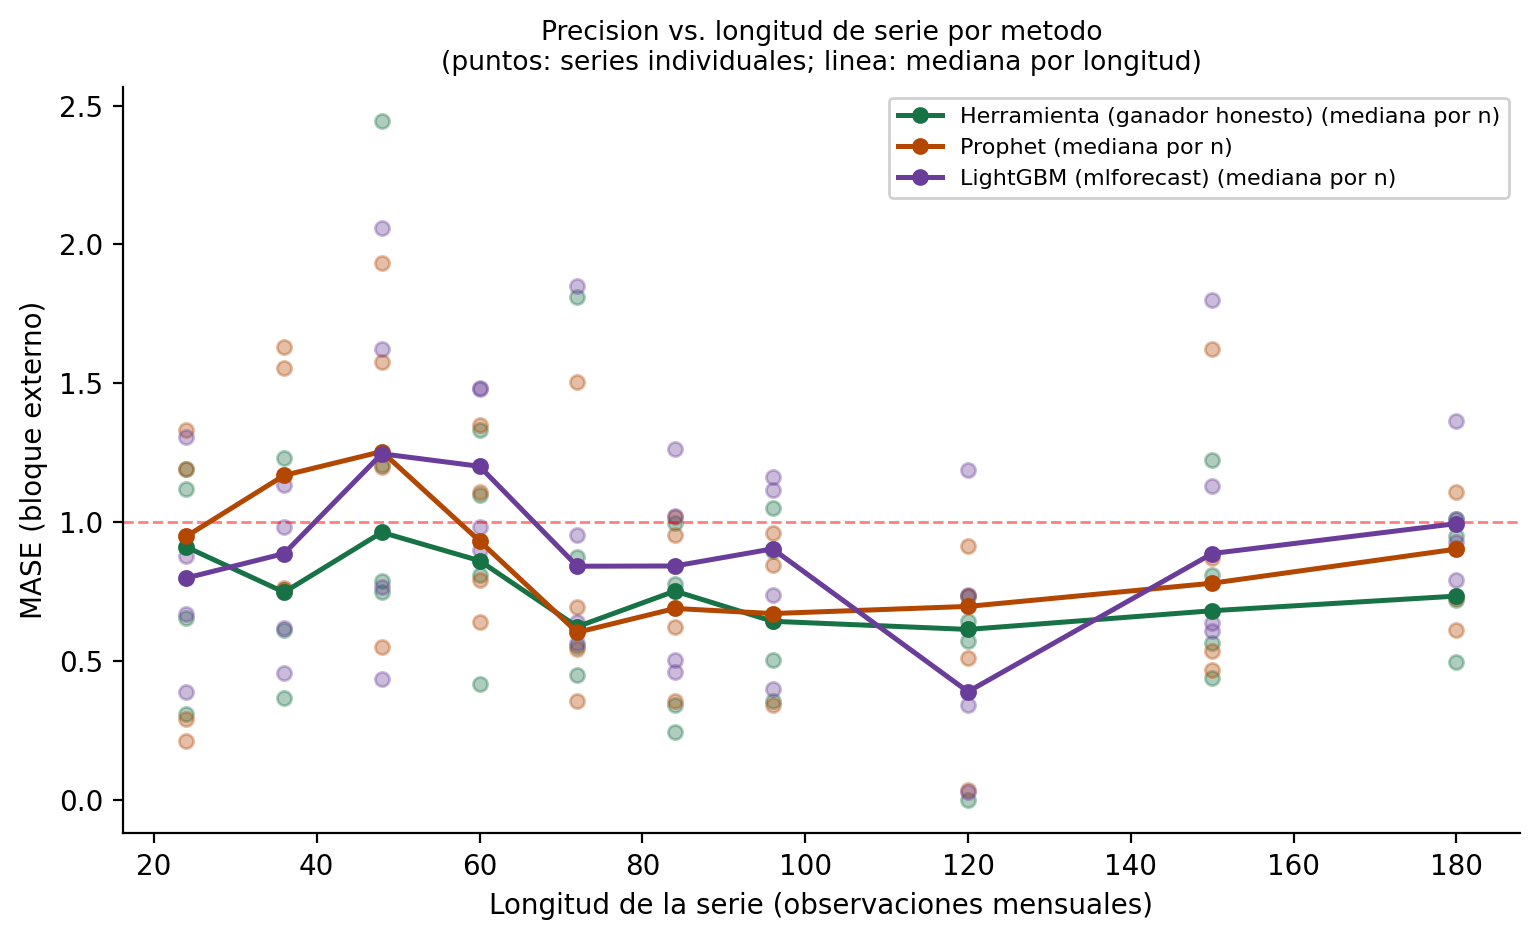
\includegraphics[width=0.85\textwidth]{figures/fig_c2_mase_vs_longitud.png}
    \caption{MASE on the held-out outer block against series length, by method (points: individual series; line: median per length). Reproducible with \texttt{codigo/experimentos/comparativa\_externa.py}.}
    \label{fig:masevslongitud}
\end{figure}

\begin{figure}[H]
    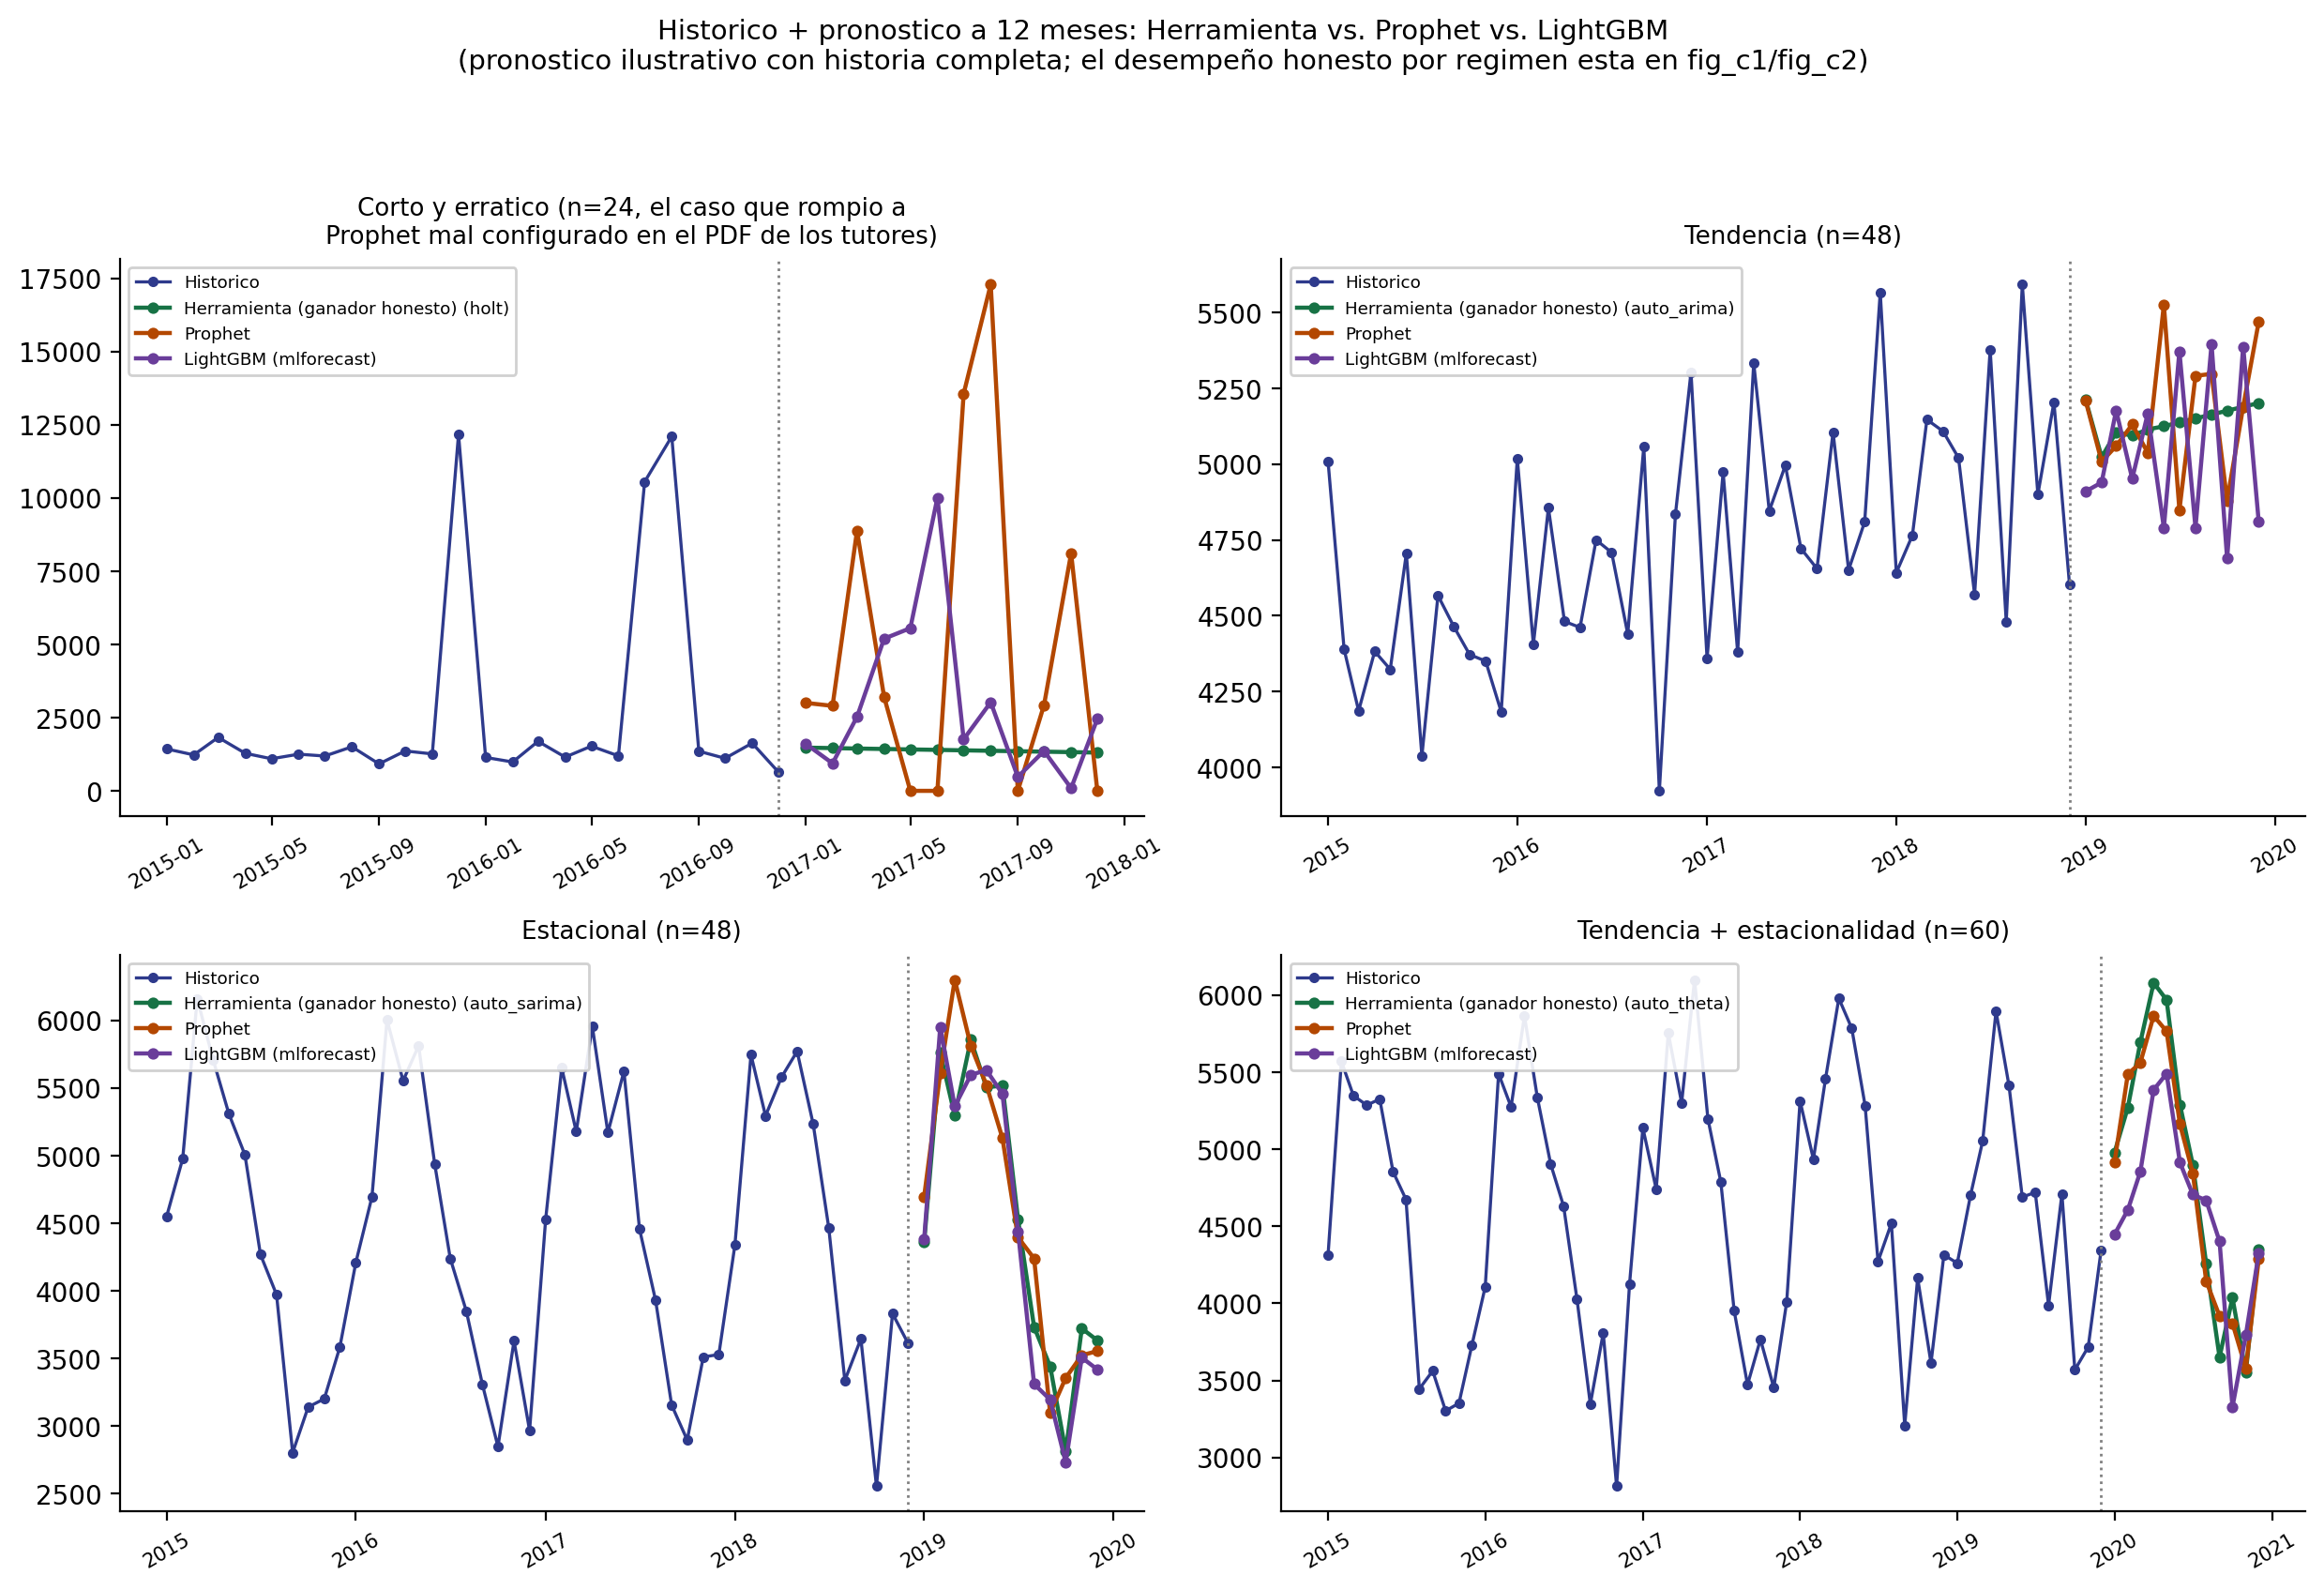
\includegraphics[width=0.85\textwidth]{figures/fig_c3_panel_regimenes.png}
    \caption{Illustrative 12-month forecast, tool vs.\ Prophet vs.\ LightGBM, on four representative structural regimes plotted over the full available history. This is a qualitative illustration of the three methods' behavior, not a substitute for the honest, external-block performance underlying it, which is reported in Table~\ref{tab:externo} and Figures~\ref{fig:boxplotmase}--\ref{fig:masevslongitud}.}
    \label{fig:panelregimenes}
\end{figure}

\begin{table}[H]
\caption{Median MASE by method, held-out outer block, synthetic panel spanning 24--180 observations ($n=$50 series). Reproducible with \texttt{codigo/experimentos/comparativa\_externa.py}.\label{tab:externo}}
\centering
\begin{tabularx}{\textwidth}{Xcccc}
\toprule
 & \textbf{Naive} & \textbf{Tool (selected method)} & \textbf{Prophet 1.4.0} & \textbf{LightGBM 4.7.0} \\
\midrule
Median MASE (all lengths) & 1.070 & 0.747 & 0.785 & 0.893 \\
Median MASE ($n=24$)      & 0.915 & 0.909 & 0.948 & \textbf{0.798} \\
Median MASE ($n=120$)     & 0.938 & 0.613 & 0.696 & \textbf{0.388} \\
Win rate vs.\ tool (all lengths) & --- & --- & 36\% & 28\% \\
\bottomrule
\end{tabularx}
\end{table}

In addition to this external comparison, the automated AICc-selected variants already integrated into the tool's own candidate pool (ARIMA, SARIMA, ETS, Theta) are evaluated alongside the classical methods at no additional dependency cost; Table~\ref{tab:ganadores} reports how often each family is selected as the winning method across the public panel of Section~\ref{sec:panel}, by structural regime, with the naive and seasonal naive benchmarks reported as separate columns rather than pooled, since a winning "benchmark" means different things for each.

\begin{table}[H]
\caption{Frequency of the winning method family by structural regime, public panel ($n=$150 series).\label{tab:ganadores}}
\centering
\begin{tabularx}{\textwidth}{Xccccc}
\toprule
\textbf{Structural regime} & \textbf{Classical} & \textbf{ARIMA/SARIMA} & \textbf{ETS/Theta} & \textbf{Naive} & \textbf{Seasonal naive} \\
\midrule
Seasonal + trend & 38\% & 24\% & 19\% & 0\% & 19\% \\
Seasonal, no trend & 19\% & 36\% & 29\% & 3\% & 13\% \\
Trend, no seasonality & 62\% & 19\% & 2\% & 17\% & 0\% \\
Flat (no trend, no seasonality) & 61\% & 23\% & 0\% & 16\% & 0\% \\
\midrule
All regimes & 49\% & 25\% & 9\% & 11\% & 5\% \\
\bottomrule
\end{tabularx}
\end{table}

Table~\ref{tab:ganadores} shows the result by regime. Across the full panel, classical smoothing or regression methods are the winning family on 49\% of series, against 34\% for an automated AICc-selected variant (25\% ARIMA/SARIMA, 9\% ETS/Theta) and 16\% for the naive or seasonal naive benchmark combined (11\% and 5\%, respectively). Automated selection is most valuable precisely where classical methods are weakest structurally: in the seasonal regimes (seasonal-plus-trend and seasonal-plain), automated ARIMA/SARIMA and ETS/Theta together win 43\% and 65\% of series respectively, more than doubling their combined share in the non-seasonal regimes (21\% and 23\%). This pattern --- simple methods remaining highly competitive overall, with automation earning its cost specifically on the more structurally demanding series --- is consistent with evidence from large-scale forecasting competitions that simple statistical methods are strong baselines in short, low-noise regimes \cite{makridakis2020}, and, together with the external comparison above, it argues for retaining classical, automated-statistical, and machine-learning candidates side by side rather than committing to any one family.

\subsection{Sensitivity Analysis of the External Comparison}
\label{sec:sensitivity}

The regime-level pattern of Table~\ref{tab:externo} and Figure~\ref{fig:masevslongitud} --- LightGBM's median MASE falling to its lowest value in the sweep at $n=120$ --- raises the question of whether the tool's relative standing against the two external comparators depends systematically on series length, rather than reflecting sampling noise from the five series available at each sampled length. This is tested with a Spearman rank correlation, computed on the full 50-series external comparison, between series length $n$ and (i) each method's own MASE and (ii) the paired tool-minus-comparator MASE difference (\texttt{codigo/experimentos/analisis\_sensibilidad\_ci.py}, reusing the \texttt{comparativa\_externa.csv} artifact of Table~\ref{tab:externo}). None of these correlations reaches conventional significance: length correlates weakly and non-significantly with the tool's own MASE ($\rho=-0.213$, $p=0.138$), with Prophet's ($\rho=-0.254$, $p=0.076$), and essentially not at all with LightGBM's ($\rho=-0.022$, $p=0.880$); the paired tool-minus-LightGBM difference is likewise uncorrelated with length ($\rho=-0.192$, $p=0.182$), as is the tool-minus-Prophet difference ($\rho=+0.062$, $p=0.666$). Read together with Figure~\ref{fig:masevslongitud}, this indicates that LightGBM's single low median at $n=120$ is consistent with sampling variability under five series per length rather than with a confirmed, monotonic length effect: the local-versus-global mechanism proposed in Section~\ref{sec:autobaselines} remains a reasonable hypothesis but this design is under-powered to confirm it directly, and a length-stratified design with more than five series per cell is the natural next step for testing it.

Percentile bootstrap 95\% confidence intervals (10,000 resamples, fixed seed) on the statistics of Table~\ref{tab:externo} add a further, specific caution for the Prophet comparison. The median paired difference (tool $-$ Prophet) is $-0.042$ MASE points, 95\% CI $[-0.115, -0.005]$, and the tool's win rate against Prophet, 95\% CI $[50\%, 78\%]$, has a lower bound at the chance level despite the point estimate (64\%) and the Wilcoxon test ($p=0.043$) both favoring the tool. The corresponding interval against LightGBM is comfortably clear of both null values (median difference $-0.134$, 95\% CI $[-0.254,-0.041]$; win rate 72\%, 95\% CI $[58\%,84\%]$). The two external comparisons are therefore not equally conclusive: the tool's advantage over LightGBM is robust under resampling, while its advantage over Prophet, though statistically significant by the Wilcoxon test, is the more fragile of the two findings in this manuscript and should be weighted accordingly in any decision that relies on it.

\begin{figure}[H]
    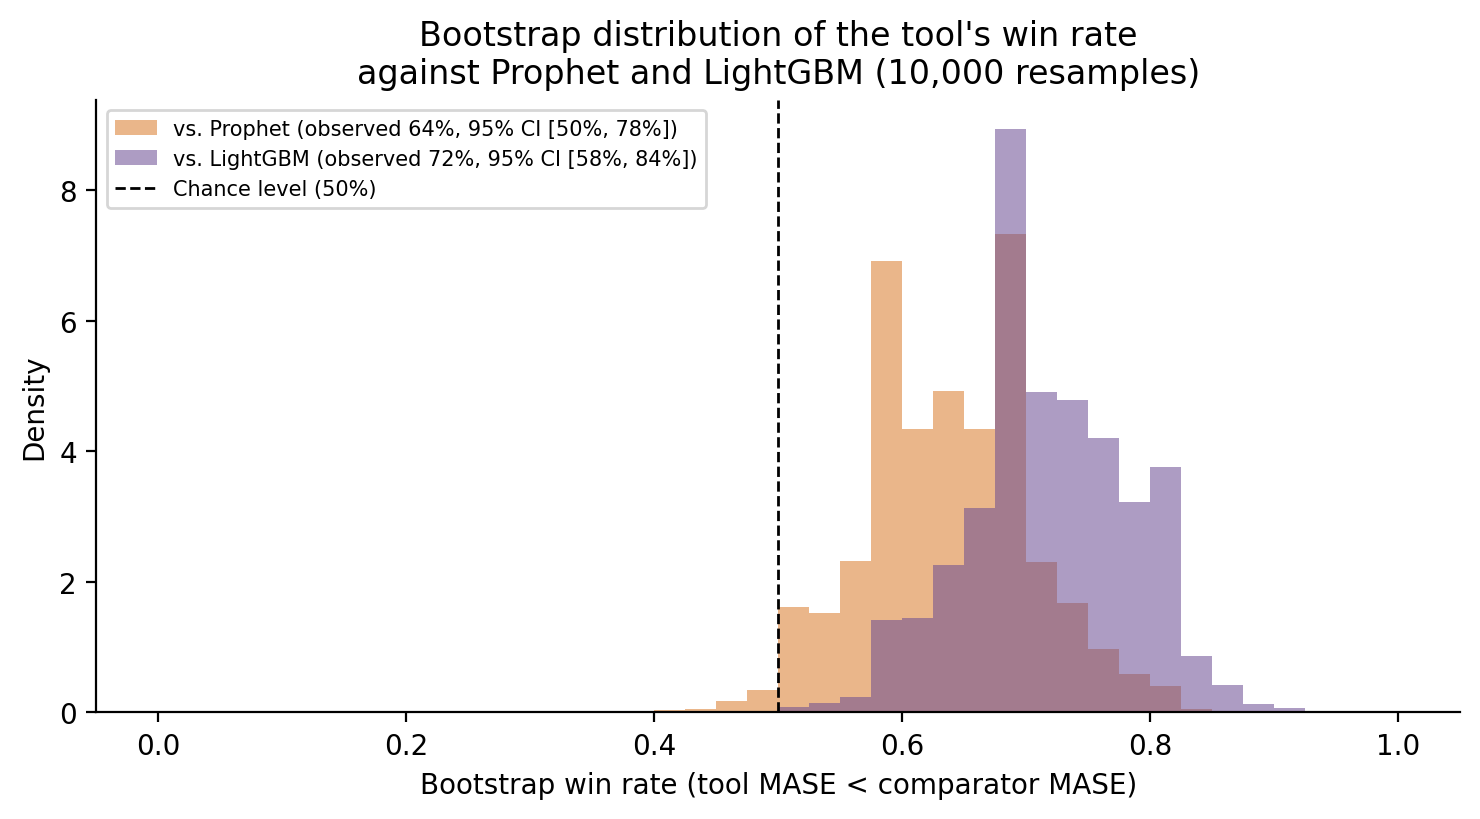
\includegraphics[width=0.85\textwidth]{figures/fig_c4_bootstrap_winrate.png}
    \caption{Bootstrap distribution (10,000 resamples) of the tool's win rate against Prophet and against LightGBM on the 50-series external comparison. The dashed line marks the 50\% chance level. The Prophet distribution's left tail reaches the chance level, while the LightGBM distribution clears it with margin.}
    \label{fig:bootstrap}
\end{figure}

\subsection{Measured Effect of Common Validation Pitfalls}
\label{sec:pitfalls}

The protocol of Section~\ref{sec:methods} is built around several specific safeguards, each aimed at one common pitfall in evaluating a forecasting tool. Rather than describing each safeguard's motivation in isolation at the point in the paper where it is introduced, this section collects, in one place, a direct measurement of how much each pitfall changes the reported conclusions when the corresponding safeguard is skipped.

\begin{itemize}
\item \textbf{Circular method-vs-benchmark comparison.} Evaluating the tool's selected method against naive on the same block that chose it among the candidates is circular: naive is one of the candidates the selection argmin runs over, so the selected method cannot lose to naive on that block by construction. On the 150-series public panel of Section~\ref{sec:panel}, this circular protocol reports a 100\% win rate against naive; the outer-block protocol used throughout this paper (Section~\ref{sec:validation}), which evaluates the selected method on origins that took no part in selecting it, reports 63\% (95 of 150 series; 17 exact ties where the tool itself selected naive; 38 losses). The 37-percentage-point gap between these two numbers is entirely an artifact of the evaluation design, not a difference in the underlying forecasts.
\item \textbf{An unsatisfiable structural filter.} An early specification of the structural filter admitted constant-level methods (simple average, moving average, weighted moving average) only when a series simultaneously satisfied $R^2 \geq 0.90$ against a linear trend fit \emph{and} $|\text{ACF}_{12}| < 0.10$ --- two conditions that are in tension by construction, since a strong linear fit and near-zero autocorrelation of the level rarely co-occur. On 3000 synthetic series spanning the structural regimes this tool targets, that criterion was satisfied by 0\% of series, meaning constant-level methods were excluded from every candidate pool regardless of whether the series actually had a stable level. The criterion used throughout this paper (Section~\ref{sec:classification}) admits constant-level methods based on the trend and stationarity tests directly, without the redundant, unsatisfiable second condition.
\item \textbf{Hyperparameter tuning on the reported evaluation block.} Selecting hyperparameters and reporting accuracy from the same walk-forward pass lets the reported metric partly reflect fit to noise in that specific block rather than genuine out-of-sample skill, a well-documented risk in time-series cross-validation \cite{bergmeir2012,tashman2000}. The tuning/evaluation split of Section~\ref{sec:hyperopt} keeps these two purposes on disjoint blocks throughout this paper.
\item \textbf{An accuracy metric undefined at zero demand.} A percentage-error metric computed as $|D_t-F_t|/\max(|D_t|,\epsilon)$ with a small numerical floor $\epsilon$ turns a zero-demand period, common in intermittent industrial series, into an arbitrarily large percentage: on one illustrative series with a single zero-demand month, this formula returns 12{,}500{,}000{,}003\%. MASE (Section~\ref{sec:metrics}) is unaffected by zero-demand periods by construction, and MAPE is reported here only over non-zero periods, with the excluded count always stated.
\item \textbf{An uncalibrated classification test.} A naive trend test (the p-value of an unweighted linear-regression slope) has a simulated false-positive rate of 74.4\% on series with no true trend; a naive seasonality test (a raw lag-12 autocorrelation threshold, which a trend inflates at every lag) has a simulated false-positive rate of 50.2\% on trending series with no true seasonality. The sequential, calibrated tests of Section~\ref{sec:classification} reduce these to a mean of 8.9\% (maximum 15.8\%) and a mean of 1.4\% (maximum 3.5\%), respectively, with unchanged power to detect a true seasonal pattern (Section~\ref{sec:methods}, Monte Carlo validation).
\end{itemize}

Two further quantities complete this account without fitting the same before/after format. First, an ablation of the structural filter itself (\texttt{codigo/experimentos/ablacion\_filtro\_estructural.py}), which reruns the same 150-series public panel of Section~\ref{sec:panel} with the filter disabled so that method selection is unconstrained by structural compatibility, isolates how much of the tool's measured performance is attributable to filtering candidates by structure specifically, as distinct from the rest of the protocol, directly answering the research question posed in the Introduction. On the identical 150 series evaluated both ways, disabling the filter changes the median MASE from 0.701 to 0.715 and the win rate against naive from 63.3\% to 62.7\% --- a small, directionally consistent degradation (about a 2\% relative increase in median MASE) rather than a large one. This indicates that structural filtering contributes a modest, measurable improvement on top of the rest of the protocol --- the tuning/evaluation split, the outer block, and mandatory benchmarks --- which together account for most of the tool's measured advantage over naive; the filter is best understood as a robustness safeguard against occasionally selecting a structurally incompatible model, not as the primary driver of accuracy. Second, because Tables~\ref{tab:incumbente} and~\ref{tab:panel} report MASE on a six-origin outer block, a sensitivity analysis (\texttt{codigo/experimentos/sensibilidad\_outer\_block.py}) reruns the same 150-series panel with the outer-block size varied across $\{6,9,12\}$ origins (Section~\ref{sec:validation}). All 150 series remain evaluable at every size. The median MASE moves from 0.701 ($n_{\text{outer}}=6$, the value used throughout this paper) to 0.707 ($n_{\text{outer}}=9$) to 0.739 ($n_{\text{outer}}=12$), and the win rate against naive moves from 63.3\% to 71.3\% to 59.3\% --- a non-monotonic pattern that is itself the point: with only 6--12 origins, a MASE estimate carries enough sampling noise that its exact value, and even whether the win rate looks stronger or weaker, depends non-trivially on how many origins happen to fall in the outer block. This confirms the concern raised in Section~\ref{sec:validation} about the sampling variance of a MASE estimate over few backtest origins, and it is the reason this paper reports a full win/tie/loss breakdown and a significance test rather than the point estimate alone; six origins was retained throughout for consistency with the smallest outer block that all three lengths of Section~\ref{sec:panel} can support, not because it produces the most favorable result --- of the three values tested here, it is neither the highest nor the lowest win rate.

\section{Discussion}
\label{sec:discussion}

The results support a narrower and more specific claim than an unqualified statement that the tool "improves accuracy." The structural filter, evaluated on the illustrative case of Section~\ref{sec:walkthrough}, behaves as intended: methods incompatible with a confirmed trend are excluded with a logged reason, consistent with feature-based model selection research showing that restricting candidates to those compatible with a series' structural features improves robustness relative to an unconstrained comparison \cite{monteromanso2020,talagala2021}. The ablation of Section~\ref{sec:pitfalls} answers the research question posed in the Introduction directly: disabling the filter on the public panel moves the median MASE by only 0.014 (0.701 to 0.715) and the win rate against naive by 0.6 percentage points, so most of the tool's measured advantage over naive is attributable to the rest of the protocol --- honest tuning/evaluation separation, the outer block, and mandatory benchmarks --- rather than to structural filtering itself, which nonetheless contributes a small, consistent improvement and functions as a robustness safeguard rather than the primary source of accuracy. At the same time, the incumbent-method comparison of Section~\ref{sec:incumbente} shows that the tool's advantage over the incumbent is not universal: on a materially sized synthetic sample reproducing the reference company's demand structure, the tool's selected method underperforms a fixed three-period moving average on a non-trivial share of series, most visibly on short, low-noise series where the incumbent's simplicity is close to optimal and where a more flexible automatically-selected model can overfit the small tuning block available. This pattern is consistent with the broader finding from large-scale forecasting competitions that simple statistical methods remain highly competitive, particularly for short, low-noise series \cite{makridakis2020}, and the same pattern recurs in the flat regime of the public-panel validation (Section~\ref{sec:panel}) and in LightGBM's competitiveness at short lengths in the external comparison (Section~\ref{sec:autobaselines}): no single method or method family is uniformly best, and the value of this protocol is in selecting among candidates under an honest evaluation, not in any one candidate being unconditionally superior. The sensitivity analysis of Section~\ref{sec:sensitivity} adds a further qualification specific to the external comparison: the tool's advantage over LightGBM survives bootstrap resampling comfortably, but its advantage over Prophet, while significant by the Wilcoxon test, has a bootstrap win-rate interval that touches the 50\% chance level, so that comparison should be read as suggestive rather than conclusive on its own.

The public-panel validation of Section~\ref{sec:panel} addresses a limitation that no single-case study can: with a large enough sample of independent series, an aggregate significance test becomes possible. Reporting a Wilcoxon signed-rank result and a full win/tie/loss breakdown alongside the median MASE, rather than a MASE figure in isolation, is what makes the regime-level heterogeneity in Table~\ref{tab:panel} --- the tool winning outright on fewer than half of flat-regime series despite a near-tied median, against clear majority wins on trending series --- visible in the first place; a single pooled accuracy figure would have hidden it.

Computational performance (Section~\ref{sec:computo}) benefits from two design choices with different character: avoiding redundant walk-forward recomputation is a pure engineering optimization with no methodological trade-off, while selecting ARIMA/SARIMA order by AICc rather than by an unconstrained grid search simultaneously reduces computational cost and removes a hyperparameter-selection bias (Section~\ref{sec:hyperopt}). That the same design choice serves both goals is not a coincidence particular to this tool: it reflects a more general point that statistically sound validation and computational efficiency are often aligned rather than in tension, contrary to a framing --- common in applied forecasting tool design --- that treats them as a trade-off to be balanced \cite{petropoulos2022}.

Several limitations remain. The tool is exclusively univariate: it does not incorporate exogenous demand drivers, such as committed order-book variables, that the reference company's own operational context suggests are informative. Forecast quality remains bounded by the available history; with fewer than roughly 36 observations, seasonality cannot be reliably identified at all (Section~\ref{sec:classification}). The trend test's own power is limited precisely in the shortest part of the regime this tool targets: at $n=24$, Monte Carlo power against a noisy linear trend is 42.7\% and against a random walk with drift is 44.2\% (0\% when a strong seasonal component is also present and not yet removed), rising to 91.4\% and 55.3\% respectively by $n=36$ and to near-100\% by $n=48$ (\texttt{resultados/montecarlo\_clasificacion.csv}); a real trend at $n=24$ is therefore as likely to be missed as detected, which the calibrated 8.9\%-mean false-positive rate of Section~\ref{sec:pitfalls} does not by itself convey. The tuning block available for hyperparameter search is correspondingly thin at short lengths, which is the most plausible explanation for the cases in Section~\ref{sec:incumbente} where the tool's selected method underperforms the incumbent. The candidate pool remains composed of classical, automated-statistical, and one machine-learning baseline (LightGBM, Section~\ref{sec:autobaselines}); it does not include deep learning architectures, which have shown competitive performance in larger-data, more complex forecasting scenarios \cite{carbonneau2008}, but whose data requirements are generally poorly matched to the 24--48 observation regime this tool targets. The public-panel validation itself has a domain-matching limitation: M3-Monthly (Section~\ref{sec:panel}) mixes micro-, industry-, and macro-level series across finance, demography, and other domains rather than being industrial demand data, and even after truncation its shortest evaluated lengths remain at the upper end (36--48 observations) of the regime this tool targets; the lower end of that regime (24--35 observations) remains validated only on the synthetic panel of Section~\ref{sec:incumbente}. These limitations define concrete, falsifiable directions for future work rather than a general caveat: acquiring real incumbent-method sales data to replace the synthetic panel of Section~\ref{sec:incumbente}, extending the exogenous-variable capability, and validating against real industrial demand series in the 24--35 observation range specifically.

\section{Conclusions}
\label{sec:conclusions}

This study developed and validated a structurally-aware, honestly-evaluated protocol and computational tool for automated demand forecasting under short, industrial-scale demand histories, and it quantified, rather than asserted, how much each element of that protocol matters. The structural classification procedure separates seasonality detection, trend detection, and stationarity testing in an order and with test specifications calibrated for short, autocorrelated demand series, reducing a naive trend test's simulated false-positive rate of 74.4\% to a mean of 8.9\% (maximum 15.8\%) and a naive seasonality test's simulated false-positive rate of 50.2\% to a mean of 1.4\% (maximum 3.5\%), against known ground truth (Section~\ref{sec:classification}, Monte Carlo validation). The validation protocol separates the block used to select hyperparameters from the block used to report performance, adds a further outer block that keeps method selection itself separate from the reported benchmark comparison, and reports mandatory naive and seasonal naive benchmarks alongside every method, without which no accuracy claim in this domain is interpretable; Section~\ref{sec:pitfalls} shows concretely how much each of these safeguards changes the reported conclusions when it is skipped.

Evaluated under this protocol, the tool's forecasting performance is real but specific rather than universal: on a synthetic panel reproducing the reference company's demand structure, evaluated on an outer block held out from both hyperparameter tuning and method selection, the tool improves on the incumbent three-period moving average by a median per-series MASE reduction of 19.9\% and outperforms it on 80\% of series, not on all of them; on an independent public panel of 150 short time series, evaluated under the same held-out protocol, it outperforms a naive benchmark on 63\% of series overall, though in the flat structural regime specifically it wins outright on fewer than half of series (45\%) despite a marginally lower median MASE. It also outperforms external Prophet and LightGBM baselines on most series across a range of lengths, though LightGBM is the strongest method at the shortest and longest lengths evaluated. The tool runs the full pipeline, including hyperparameter tuning, in on the order of tens of seconds for series of up to 120 monthly observations on a constrained consumer hardware profile (Section~\ref{sec:computo}, where repeated measurement shows this figure is noisy but consistently well within a one-minute budget), and comfortably within the 25-second interactive-session target for the shorter series (up to 48 observations) this tool primarily targets.

The practical contribution is a fully reproducible, tested, open-source computational framework that automates structurally-aware forecasting for short industrial demand histories, including prediction intervals and derived inventory-policy parameters that close the gap between a point forecast and a stock-management decision. The academic contribution is methodological: a validation protocol for this regime together with a direct, quantified account of how much each of its individual safeguards --- structural filtering, the tuning/evaluation split, the outer block, mandatory benchmarks, and a zero-robust accuracy metric --- changes the reported conclusions when it is skipped (Section~\ref{sec:pitfalls}), backed by a test suite that verifies each safeguard does not silently regress. Future work should prioritize validating the tool against the reference company's real historical sales records once available, extending the candidate pool to intermittent-demand-specific methods for the zero-inflated series this industrial context produces, and incorporating exogenous demand drivers tied to committed order-book activity.

%%%%%%%%%%%%%%%%%%%%%%%%%%%%%%%%%%%%%%%%%%
%%%%%%%%%%%%%%%%%%%%%%%%%%%%%%%%%%%%%%%%%%
\vspace{6pt} 

%%%%%%%%%%%%%%%%%%%%%%%%%%%%%%%%%%%%%%%%%%
%% optional
%\supplementary{The following supporting information can be downloaded at:  \linksupplementary{s1}, Figure S1: title; Table S1: title; Video S1: title.}

% Only for journal Methods and Protocols:
% If you wish to submit a video article, please do so with any other supplementary material.
% \supplementary{The following supporting information can be downloaded at: \linksupplementary{s1}, Figure S1: title; Table S1: title; Video S1: title. A supporting video article is available at doi: link.}

% Only used for preprtints:
% \supplementary{The following supporting information can be downloaded at the website of this paper posted on \href{https://www.preprints.org/}{Preprints.org}.}

% Only for journal Hardware:
% If you wish to submit a video article, please do so with any other supplementary material.
% \supplementary{The following supporting information can be downloaded at: \linksupplementary{s1}, Figure S1: title; Table S1: title; Video S1: title.\vspace{6pt}\\
%\begin{tabularx}{\textwidth}{lll}
%\toprule
%\textbf{Name} & \textbf{Type} & \textbf{Description} \\
%\midrule
%S1 & Python script (.py) & Script of python source code used in XX \\
%S2 & Text (.txt) & Script of modelling code used to make Figure X \\
%S3 & Text (.txt) & Raw data from experiment X \\
%S4 & Video (.mp4) & Video demonstrating the hardware in use \\
%... & ... & ... \\
%\bottomrule
%\end{tabularx}
%}

%%%%%%%%%%%%%%%%%%%%%%%%%%%%%%%%%%%%%%%%%%
\authorcontributions{Conceptualization, C.V.G., L.T.-T.\ and D.\'A.-M.; methodology, C.V.G., J.J.S.-A., L.T.-T.\ and D.\'A.-M.; software, C.V.G., J.J.S.-A.\ and M.P.C.R.; validation, C.V.G., J.J.S.-A., M.P.C.R.\ and L.T.-T.; formal analysis, C.V.G., J.J.S.-A.\ and D.\'A.-M.; investigation, C.V.G., J.J.S.-A.\ and M.P.C.R.; resources, L.T.-T.\ and D.\'A.-M.; data curation, C.V.G., J.J.S.-A.\ and M.P.C.R.; writing---original draft preparation, C.V.G., J.J.S.-A.\ and M.P.C.R.; writing---review and editing, L.T.-T.\ and D.\'A.-M.; visualization, C.V.G.\ and M.P.C.R.; supervision, L.T.-T.\ and D.\'A.-M.; project administration, L.T.-T. All authors have read and agreed to the published version of the manuscript.}

\funding{This research received no external funding.}

\institutionalreview{Not applicable. This study did not involve human participants or animals; it analyzes a synthetic demand panel that reproduces the structural characteristics of a reference company's process (no company sales records are used quantitatively) and a publicly available benchmark time series panel.}

\informedconsent{Not applicable.}

\dataavailability{The forecasting package, application, test suite, and all reproducibility scripts used to generate the results in Section~\ref{sec:results} are available at \url{https://github.com/GIUSEPPESAN21/Forecasting} (see Section~\ref{sec:availability} for details). The reference company's historical sales records underlying the diagnosis of Section~\ref{sec:diagnosis} are proprietary and are not publicly available due to commercial confidentiality; a synthetic panel reproducing the same structural characteristics is provided in the repository so that all analysis scripts run end to end without access to any company's data. The public M3-Monthly panel used in Section~\ref{sec:panel} is available from its original source \cite{makridakis2020m3} and is downloaded automatically by the corresponding script.}

%\durcstatement{Current research is limited to the [please insert a specific academic field, e.g., XXX], which is beneficial [share benefits and/or primary use] and does not pose a threat to public health or national security. Authors acknowledge the dual-use potential of the research involving xxx and confirm that all necessary precautions have been taken to prevent potential misuse. As an ethical responsibility, authors strictly adhere to relevant national and international laws about DURC. Authors advocate for responsible deployment, ethical considerations, regulatory compliance, and transparent reporting to mitigate misuse risks and foster beneficial outcomes.}

% Only for journal Nursing Reports
%\publicinvolvement{Please describe how the public (patients, consumers, carers) were involved in the research. Consider reporting against the GRIPP2 (Guidance for Reporting Involvement of Patients and the Public) checklist. If the public were not involved in any aspect of the research add: ``No public involvement in any aspect of this research''.}
%
%% Only for journal Nursing Reports
%\guidelinesstandards{Please add a statement indicating which reporting guideline was used when drafting the report. For example, ``This manuscript was drafted against the XXX (the full name of reporting guidelines and citation) for XXX (type of research) research''. A complete list of reporting guidelines can be accessed via the equator network: \url{https://www.equator-network.org/}.}
%
%% Only for journal Nursing Reports
%\useofartificialintelligence{Please describe in detail any and all uses of artificial intelligence (AI) or AI-assisted tools used in the preparation of the manuscript. This may include, but is not limited to, language translation, language editing and grammar, or generating text. Alternatively, please state that “AI or AI-assisted tools were not used in drafting any aspect of this manuscript”.}

\acknowledgments{The authors thank the reference company for providing access to its historical forecasting process for the diagnosis reported in Section~\ref{sec:diagnosis}. During the preparation of this manuscript, the authors used Claude (Anthropic) to assist in implementing the forecasting pipeline, running the reproducibility scripts underlying Section~\ref{sec:results}, and drafting portions of the manuscript text, as detailed in Section~\ref{sec:genai}. The authors have reviewed and edited the output and take full responsibility for the content of this publication.}

\conflictsofinterest{The authors declare no conflicts of interest. The reference company had no role in the design of the study, in the collection, analysis, or interpretation of data, in the writing of the manuscript, or in the decision to publish the results.}

%%%%%%%%%%%%%%%%%%%%%%%%%%%%%%%%%%%%%%%%%%
%% Optional

%% Only for journal Encyclopedia
%\entrylink{The Link to this entry published on the encyclopedia platform.}

\abbreviations{Abbreviations}{
The following abbreviations are used in this manuscript:
\\

\noindent
\begin{tabular}{@{}ll}
ADF & Augmented Dickey--Fuller (test)\\
AICc & Corrected Akaike Information Criterion\\
ARIMA & Autoregressive Integrated Moving Average\\
ETS & Error, Trend, Seasonal (exponential smoothing family)\\
KPSS & Kwiatkowski--Phillips--Schmidt--Shin (test)\\
MAD & Mean Absolute Deviation\\
MAPE & Mean Absolute Percentage Error\\
MASE & Mean Absolute Scaled Error\\
ME & Mean Error\\
MDPI & Multidisciplinary Digital Publishing Institute\\
MSE & Mean Squared Error\\
SARIMA & Seasonal Autoregressive Integrated Moving Average\\
SES & Simple Exponential Smoothing\\
SKU & Stock-Keeping Unit\\
STL & Seasonal-Trend decomposition using Loess
\end{tabular}
}

%%%%%%%%%%%%%%%%%%%%%%%%%%%%%%%%%%%%%%%%%%
% No appendix: every table and figure in this manuscript is cited in the main
% text, and all supplementary material (test suite, experiment scripts, and
% their output) is referenced via the repository in Section~\ref{sec:availability}.
%%%%%%%%%%%%%%%%%%%%%%%%%%%%%%%%%%%%%%%%%%
%\isPreprints{}{% This command is only used for ``preprints''.
\begin{adjustwidth}{-\extralength}{0cm}
%} % If the paper is ``preprints'', please uncomment this parenthesis.
%\printendnotes[custom] % Un-comment to print a list of endnotes

\reftitle{References}

% Please provide the correct journal abbreviation (e.g. according to the “List of Title Word Abbreviations” http://www.issn.org/services/online-services/access-to-the-ltwa/).
% Citations and References in Supplementary files are permitted provided that they also appear in the reference list here. 

%=====================================
% References, variant A: external bibliography
%=====================================
% \bibliography{your_external_BibTeX_file}

%=====================================
% References, variant B: internal bibliography
%=====================================

% Numeric (ACS) format, as required for the journal Forecasting.
% Every entry below corresponds to a verifiable publication; none was
% generated or approximated by the GenAI system used in this revision
% (Section~\ref{sec:genai}). 36 entries.
\begin{thebibliography}{99}

\bibitem{mentzer2001}
Moon, M.A.; Mentzer, J.T.; Smith, C.D. Conducting a sales forecasting audit. \textit{Int. J. Forecast.} \textbf{2003}, \textit{19}, 5--25.

\bibitem{chopra2021}
Chopra, S.; Meindl, P. \textit{Supply Chain Management: Strategy, Planning, and Operation}, 7th ed.; Pearson: Harlow, UK, 2019.

\bibitem{makridakis1998}
Makridakis, S.; Wheelwright, S.C.; Hyndman, R.J. \textit{Forecasting: Methods and Applications}, 3rd ed.; John Wiley \& Sons: New York, NY, USA, 1998.

\bibitem{hyndman2021}
Hyndman, R.J.; Athanasopoulos, G. \textit{Forecasting: Principles and Practice}, 3rd ed.; OTexts: Melbourne, Australia, 2021.

\bibitem{ballou2004}
Ballou, R.H. \textit{Business Logistics/Supply Chain Management: Planning, Organizing, and Controlling the Supply Chain}, 5th ed.; Pearson Prentice Hall: Upper Saddle River, NJ, USA, 2004.

\bibitem{silver1998}
Silver, E.A.; Pyke, D.F.; Peterson, R. \textit{Inventory Management and Production Planning and Scheduling}, 3rd ed.; John Wiley \& Sons: New York, NY, USA, 1998.

\bibitem{syntetos2005}
Syntetos, A.A.; Boylan, J.E. The accuracy of intermittent demand estimates. \textit{Int. J. Forecast.} \textbf{2005}, \textit{21}, 303--314.

\bibitem{sattar2025}
Sattar, M.U.; Dattana, V.; Hasan, R.; Mahmood, S.; Khan, H.W.; Hussain, S. Enhancing supply chain management: A comparative study of machine learning techniques with cost--accuracy and ESG-based evaluation for forecasting and risk mitigation. \textit{Sustainability} \textbf{2025}, \textit{17}, 5772.

\bibitem{nahmias2015}
Nahmias, S.; Olsen, T.L. \textit{Production and Operations Analysis}, 7th ed.; Waveland Press: Long Grove, IL, USA, 2015.

\bibitem{kerkkanen2009}
Kerkk\"{a}nen, A.; Korpela, J.; Huiskonen, J. Demand forecasting errors in industrial context: Measurement and impacts. \textit{Int. J. Prod. Econ.} \textbf{2009}, \textit{118}, 43--48.

\bibitem{makridakis2018}
Makridakis, S.; Spiliotis, E.; Assimakopoulos, V. Statistical and machine learning forecasting methods: Concerns and ways forward. \textit{PLoS ONE} \textbf{2018}, \textit{13}, e0194889.

\bibitem{makridakis2020}
Makridakis, S.; Spiliotis, E.; Assimakopoulos, V. The M4 Competition: 100,000 time series and 61 forecasting methods. \textit{Int. J. Forecast.} \textbf{2020}, \textit{36}, 54--74.

\bibitem{makridakis2020m3}
Makridakis, S.; Hibon, M. The M3-Competition: Results, conclusions and implications. \textit{Int. J. Forecast.} \textbf{2000}, \textit{16}, 451--476.

\bibitem{monteromanso2020}
Montero-Manso, P.; Athanasopoulos, G.; Hyndman, R.J.; Talagala, T.S. FFORMA: Feature-based forecast model averaging. \textit{Int. J. Forecast.} \textbf{2020}, \textit{36}, 86--92.

\bibitem{talagala2021}
Talagala, T.S.; Hyndman, R.J.; Athanasopoulos, G. Meta-learning how to forecast time series. \textit{J. Forecast.} \textbf{2023}, \textit{42}, 1476--1501.

\bibitem{carbonneau2008}
Carbonneau, R.; Laframboise, K.; Vahidov, R. Application of machine learning techniques for supply chain demand forecasting. \textit{Eur. J. Oper. Res.} \textbf{2008}, \textit{184}, 1140--1154.

\bibitem{maack2024}
Maack, R.G.C.; Raith, F.; P\'{e}rez, J.F.; Scheuermann, G.; Gillmann, C. A workflow to systematically design uncertainty-aware visual analytics applications. \textit{Vis. Comput.} \textbf{2025}, \textit{41}, 1485--1498. (Published online 2024.)

\bibitem{hernandez2025}
Hernandez, J.E.B.; Torres, L.E.T.; Tabares, A.; \'{A}lvarez-Mart\'{i}nez, D. Optimization of bus dispatching in public transportation through a heuristic approach based on passenger demand forecasting. \textit{Smart Cities} \textbf{2025}, \textit{8}, 87.

\bibitem{nunez2024}
N\'{u}\~{n}ez-Oviedo, M.; Tarazona-Torres, L. Gesti\'{o}n de inventarios de una compa\~{n}\'{i}a importadora de repuestos de transmisi\'{o}n de potencia de maquinaria pesada. \textit{Ing. Ind.} \textbf{2024}, \textit{47}, 79--102.

\bibitem{cubides2025}
Cubides, C.S.P.; Tarazona-Torres, L. Planificaci\'{o}n agregada para el transporte de personal y materiales en el sector hidrocarburos. \textit{Ing. Ind.} \textbf{2025}, \textit{48}, 39--62.

\bibitem{bergmeir2012}
Bergmeir, C.; Ben\'{i}tez, J.M. On the use of cross-validation for time series predictor evaluation. \textit{Inf. Sci.} \textbf{2012}, \textit{191}, 192--213.

\bibitem{tashman2000}
Tashman, L.J. Out-of-sample tests of forecasting accuracy: An analysis and review. \textit{Int. J. Forecast.} \textbf{2000}, \textit{16}, 437--450.

\bibitem{hyndmankoehler2006}
Hyndman, R.J.; Koehler, A.B. Another look at measures of forecast accuracy. \textit{Int. J. Forecast.} \textbf{2006}, \textit{22}, 679--688.

\bibitem{wang2006}
Wang, X.; Smith, K.A.; Hyndman, R.J. Characteristic-based clustering for time series data. \textit{Data Min. Knowl. Discov.} \textbf{2006}, \textit{13}, 335--364.

\bibitem{ollechwebel2020}
Ollech, D.; Webel, K. A random forest-based approach to combining and ranking seasonality tests. \textit{J. Econom. Methods} \textbf{2023}, \textit{12}, 117--130.

\bibitem{kruskal1952}
Kruskal, W.H.; Wallis, W.A. Use of ranks in one-criterion variance analysis. \textit{J. Am. Stat. Assoc.} \textbf{1952}, \textit{47}, 583--621.

\bibitem{dickeyfuller1979}
Dickey, D.A.; Fuller, W.A. Distribution of the estimators for autoregressive time series with a unit root. \textit{J. Am. Stat. Assoc.} \textbf{1979}, \textit{74}, 427--431.

\bibitem{cochraneorcutt1949}
Cochrane, D.; Orcutt, G.H. Application of least squares regression to relationships containing autocorrelated error terms. \textit{J. Am. Stat. Assoc.} \textbf{1949}, \textit{44}, 32--61.

\bibitem{neweywest1987}
Newey, W.K.; West, K.D. A simple, positive semi-definite, heteroskedasticity and autocorrelation consistent covariance matrix. \textit{Econometrica} \textbf{1987}, \textit{55}, 703--708.

\bibitem{kpss1992}
Kwiatkowski, D.; Phillips, P.C.B.; Schmidt, P.; Shin, Y. Testing the null hypothesis of stationarity against the alternative of a unit root. \textit{J. Econom.} \textbf{1992}, \textit{54}, 159--178.

\bibitem{hyndmankhandakar2008}
Hyndman, R.J.; Khandakar, Y. Automatic time series forecasting: The forecast package for R. \textit{J. Stat. Softw.} \textbf{2008}, \textit{27}, 1--22.

\bibitem{garza2022}
Garza, F.; Canseco, M.M.; Challu, C.; Olivares, K.G. \textit{StatsForecast: Lightning Fast Forecasting with Statistical and Econometric Models}; Nixtla: San Francisco, CA, USA, 2022. Available online: \url{https://github.com/Nixtla/statsforecast} (accessed on 24 August 2026).

\bibitem{taylorletham2018}
Taylor, S.J.; Letham, B. Forecasting at scale. \textit{Am. Stat.} \textbf{2018}, \textit{72}, 37--45.

\bibitem{garza2022mlforecast}
Nixtla. \textit{mlforecast: Scalable Machine Learning for Time Series Forecasting}; Nixtla: San Francisco, CA, USA, 2022. Available online: \url{https://github.com/Nixtla/mlforecast} (accessed on 24 August 2026).

\bibitem{ke2017lightgbm}
Ke, G.; Meng, Q.; Finley, T.; Wang, T.; Chen, W.; Ma, W.; Ye, Q.; Liu, T.-Y. LightGBM: A highly efficient gradient boosting decision tree. In \textit{Advances in Neural Information Processing Systems 30 (NIPS 2017)}; Curran Associates: Red Hook, NY, USA, 2017; pp. 3146--3154.

\bibitem{petropoulos2022}
Petropoulos, F.; Apiletti, D.; Assimakopoulos, V.; Babai, M.Z.; Barrow, D.K.; Ben Taieb, S.; Bergmeir, C.; Bessa, R.J.; Bijak, J.; Boylan, J.E.; et al. Forecasting: Theory and practice. \textit{Int. J. Forecast.} \textbf{2022}, \textit{38}, 705--871.

\end{thebibliography}

% If authors have biography, please use the format below
%\section*{Short Biography of Authors}
%\bio
%{\raisebox{-0.35cm}{\includegraphics[width=3.5cm,height=5.3cm,clip,keepaspectratio]{Definitions/author1.pdf}}}
%{\textbf{Firstname Lastname} Biography of first author}
%
%\bio
%{\raisebox{-0.35cm}{\includegraphics[width=3.5cm,height=5.3cm,clip,keepaspectratio]{Definitions/author2.jpg}}}
%{\textbf{Firstname Lastname} Biography of second author}

%%%%%%%%%%%%%%%%%%%%%%%%%%%%%%%%%%%%%%%%%%
%% for journal Sci
%\reviewreports{\\
%Reviewer 1 comments and authors’ response\\
%Reviewer 2 comments and authors’ response\\
%Reviewer 3 comments and authors’ response
%}
%%%%%%%%%%%%%%%%%%%%%%%%%%%%%%%%%%%%%%%%%%
\PublishersNote{}
%\isPreprints{}{% This command is only used for ``preprints''.
\end{adjustwidth}
%} % If the paper is ``preprints'', please uncomment this parenthesis.
\end{document}

